\documentclass[a4paper, 12pt]{article}
\usepackage[T1]{fontenc}
\usepackage{lmodern}
\usepackage{color}
\usepackage{amsfonts}
\usepackage{epstopdf}
\usepackage{matlab}
\usepackage{booktabs}
%\documentclass{book}
\usepackage{blindtext}
\usepackage{hyperref}
\usepackage[brazil]{babel}
\usepackage{amssymb}
\usepackage[utf8]{inputenc}
\usepackage{amsmath}
\usepackage{indentfirst}
\usepackage{graphicx}
\usepackage{listings}
\usepackage{tcolorbox}
\usepackage{upgreek}
\usepackage{multicol,lipsum}
\usepackage[a4paper,
top=3cm, left=3cm, bottom=3cm, right=3cm]{geometry}
\usepackage{setspace}
\usepackage{multirow}
\usepackage{float}
\usepackage[dvipsnames]{xcolor}
\usepackage[table]{xcolor}
%\usepackage{pdflscape}
\usepackage[DIV=15]{typearea}
\usepackage[nottoc]{tocbibind}
\usepackage[sort,numbers]{natbib}
%\usepackage{cite}
\usepackage{matlab}

\usepackage[utf8]{inputenc}
\usepackage[T1]{fontenc}
\usepackage{lmodern}
\usepackage{graphicx}
\usepackage{color}
\usepackage{hyperref}
\usepackage{amsmath}
\usepackage{amsfonts}
\usepackage{epstopdf}
\usepackage[table]{xcolor}
\usepackage{matlab}

\lstdefinestyle{python}{
  language=Python,
  basicstyle=\ttfamily,
  keywordstyle=\color{blue},
  stringstyle=\color{orange},
  commentstyle=\color{gray},
  numbers=left,
  numberstyle=\tiny\color{gray},
  stepnumber=1,
  numbersep=5pt,
  backgroundcolor=\color{white},
  showspaces=false,
  showstringspaces=false,
  showtabs=false,
  frame=single,
  rulecolor=\color{black},
  tabsize=4,
  captionpos=b,
  breaklines=true,
  breakatwhitespace=false,
  title=\lstname,
  escapeinside={\%*}{*)},
  morekeywords={self},
  emph={MyClass,__init__},
  emphstyle=\color{red}
}


\documentclass[letterpaper]{article}
% bib pack %%%%%%%%%%%%%%%%%%%%%%%%%%%%%%%%%%%%%%%%%%%%%%%%%%%%%%%%%%%%%%%%%%%%%
\usepackage[utf8]{inputenc}
\usepackage{geometry}
    \geometry{left=3cm,right=2cm,top=2cm,bottom=2cm}
%
\usepackage[spanish]{babel}
%
\usepackage[fixlanguage]{babelbib}
    \bibliographystyle{babunsrt}
%
\usepackage{url}

\begin{document}
%\maketitle

\begin{titlepage}
	\begin{center}
		

\vspace{10pt}
%\begin{figure}[H][!ht]
%\centering
%
\includegraphics{puc-rio-logo.png}

%\end{figure}
\begin{figure}[!ht]
\centering

\includegraphics{images/puc-rio-logo.png}
\end{figure}
\huge{Análise de Séries Temporais}
        \vspace{70pt}
        
		\textbf{ENG1469}
		\textbf{\large{\\ }}
		
		\vspace{30pt}
		\textbf{\small{\\Lista Prática 03}}
		\vspace{75pt}
		
	\end{center}
	
	\begin{flushleft}
		\begin{tabbing}
		Aluno(a)\qquad\qquad\=\>Paloma Fernanda Loureiro Sette - 1621595\\
			Professor(a)\>Cristiano Fernandes\\
	\end{tabbing}
		  
	\end{flushleft}
	\begin{center}
		%\vspace{\fill}
		\vspace{215pt}
		Rio de Janeiro, 24 de Novembro de 2024
	\end{center}
\end{titlepage}
%%%%%%%%%%%%%%%%%%%%%%%%%%%%%%%%%%%%%%%%%%%%%%%%%%%%%%%%%%%
\newpage
\tableofcontents
\thispagestyle{empty}

\newpage
\pagenumbering{arabic}

\newpage

%\newcommand{\listequationsname}{Lista de Equações}
%\newlistof{myequations}{equ}{\listequationsname}
%\newcommand{\myequations}[1]{%
%\addcontentsline{equ}{myequations}{\protect\numberline{\theequation}#1}\par}

%\listofmyequations
\newpage


\newpage

\listoffigures
\thispagestyle{empty}

\newpage
%%%%%%%%%%%%%%%%%%%%%%%%%%%%%%%%%%%%%%%%%%%%%%%%%%%%%%%%%
%%%%%%%%%%%%%%%%%%%%%%%%%%%%%%%%%%%%%%%%%%%%%%%%%%%

\newpage

\thispagestyle{empty}

\newpage

\section*{Introdução}
Este relatório refere-se à terceira lista prática da disciplina de Análise de Séries Temporais (ENG1469) de 2024.2.\\

Para este trabalho, continuaremos a utilizar a série temporal relacionada a vendas nominais no varejo de livros, jornais, revistas e papelaria. É possível encontrar esta série no \href{http://ipeadata.gov.br/Default.aspx}{Ipeadata}. (macroeconômico >> Periodicidade >> Mensal >> Consumo e Vendas >> Vendas nominais no varejo de livros, jornais, revistas e papelaria). Abaixo, apresentamos uma breve demonstração de como chegar até a base de dados utilizada. Esta demonstração se deve ao fato de que, por algum motivo, o site do Ipeadata não nos gera o link exato até a base (ou seja, qualquer endereço que copiamos é sempre http://ipeadata.gov.br/Default.aspx).\\



\begin{figure}[H]
\centering
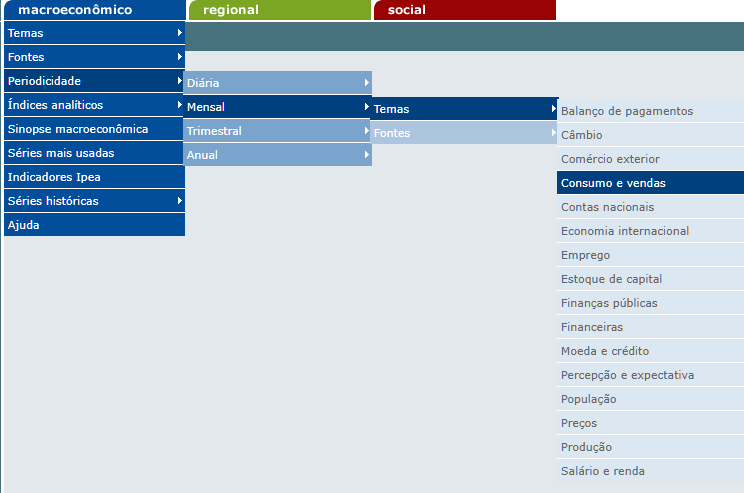
\includegraphics[scale = 0.65]{images/caminho_ipeadata.png}
\label{filtro1}
\caption{Ipeadata - caminho até a base de dados}
\end{figure}

\begin{figure}[H]
\centering
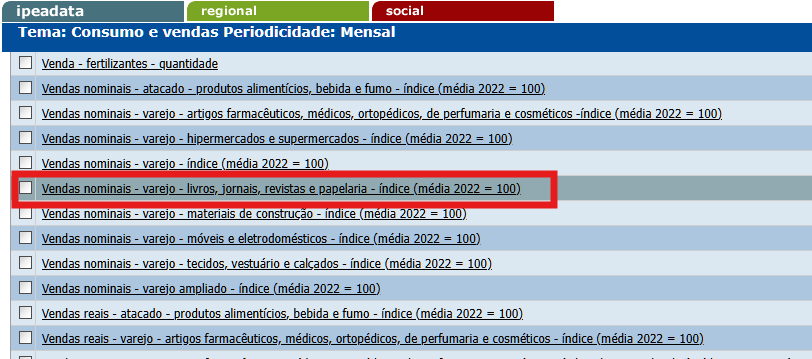
\includegraphics[scale = 0.65]{images/ipeadata_caminho2.png}
\label{filtro1}
\caption{Ipeadata - base de dados utilizada}
\end{figure}

Para vendas nominais, considera-se a receita bruta de revenda, total e por Unidade da Federação, definida no âmbito da empresa como a receita bruta mensal proveniente da revenda de mercadorias, não deduzidos os impostos incidentes e nem as vendas canceladas, abatimentos e impostos incondicionais. Para varejo considera-se as atividades de revenda, venda sem transformação significativa, de bens de consumo novos e usados, preponderantemente para o consumidor final. O comércio varejista é organizado para vender mercadorias em pequenas quantidades ao consumidor final, representando, portanto, o último elo da cadeia de distribuição. A classificação das atividades do comércio varejista baseia-se na gama de produtos vendidos, sem distinção da forma de comercialização em loja ou fora de loja. Para livros, jornais, revistas e papelaria considera-se o comércio varejista de livros, inclusive didáticos, o comércio varejista de revistas, jornais, revistas e outros impressos, o comércio varejista de artigos de escritório, as bancas de jornais e revistas, o comércio varejista de artigos de papelaria, tais como cadernos, borrachas, lápis, canetas, cartolinas e similares. Não fazendo parte desta classificação o comercio varejista de livros usados, o comércio varejista de selos, o comércio varejista de suprimentos de informática. A base foi fixada como a média das observações no ano de 2022. Nota: A Pesquisa Mensal de Comércio foi iniciada em janeiro de 1995, com o intuito de produzir indicadores que possam acompanhar o desempenho conjuntural do comércio varejista no país, investigando a receita bruta de revenda nas empresas formalmente constituídas de 20 ou mais pessoas ocupadas.\\

\newpage
\subsection{Carregando os dados}
A princípio, é necessário carregar os dados e fazer os devidos tratamentos:

\begin{lstlisting}[style=python]
import pandas as pd

file_path = 'dados.xls' 

data = pd.read_excel(file_path)

data['Data'] = data['Data'].astype(str)

data['Data'] = pd.to_datetime(data['Data'], format='%Y.%m')

data.set_index('Data', inplace=True)

# Dividindo a serie em treino e teste
train = data.iloc[:-12]  # Todas as observacoes exceto as 12 ultimas
test = data.iloc[-12:]   # As ultimas 12 observacoes

\end{lstlisting} \\

No código acima, carregamos os dados do documento XLS original, que contém as colunas Data e Vendas, e dividimos a série em dados de treino e teste. 

\begin{figure}[H]
\centering
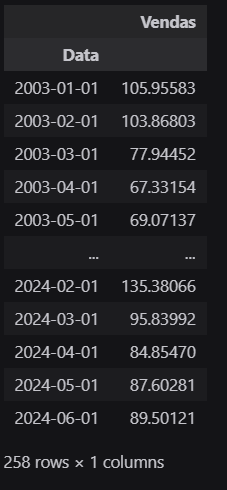
\includegraphics[scale = 0.80]{images/0.1.png}
\label{filtro1}
\caption{Dataframe base - ST}
\end{figure}

\newpage
\subsection{Especificações}

Para melhor especificar os dados da série, implementamos a tabela abaixo, cujos dados referem-se a:

\begin{itemize}
    \item Data do início e do fim;
    \item Data de início e fim do período de treinamento;
    \item Data de início e fim do período de teste;
    \item Unidade de medida;
    \item Fonte de dados.
\end{itemize}

\begin{table}[htbp]
\centering
\begin{tabular}{|l|l|}
\hline
\textbf{Descrição}                                        & \textbf{Detalhes}                    \\ \hline
Data de início e fim da série                             & 2003-01-01 - 2024-06-01              \\ \hline
Data de início e fim do período de treinamento            & 2003-01-01 - 2023-06-01              \\ \hline
Data de início e fim do período de teste                  & 2023-06-01 - 2024-06-01              \\ \hline
Unidade de medida                                          & Índice (média 2022 = 100)            \\ \hline
Fonte de dados                                             & IPEADATA                             \\ \hline
\end{tabular}
\caption{Especificações da Série Temporal}
\end{table}




%%%%%%%%%%%%%%%%%%%%%%%%%%%%%%%%%%%%%%%%%%%%%%%%%
\newpage
\section{Primeira Questão}

\subsection{Parte (a)}
\textit{\textbf{Enunciado}: Estime um modelo SARIMA à sua série original, utilizando o auto.arima (esse modelo
deve coincidir com o modelo ótimo estimado no trabalho 02). Especifique a equação
SARIMA(p,d,q)(P,D,Q), identificando as ordens p, q, d, D, P e Q para esse modelo.}\\

No trabalho 2, havíamos ajustado um novo modelo SARIMA com sazonalidade habilitada permitindo que o procedimento escolhesse automaticamente os valores de $d$ (ordem de integração não-sazonal) e $D$ (ordem de integração sazonal). Neste caso, o melhor modelo encontrado havia sido o $SARIMA(3,1,1)(1,0,1)_{12}$. Reestimando o modelo:\\

\begin{lstlisting}[style=python]
    """ QUESTAO 01"""
### Parte (a)

# Ajustar o modelo ARIMA nao-sazonal com base no AICc
model = pm.auto_arima(train['Vendas'],
                      start_p=0, max_p=5,
                      start_q=0, max_q=5,
                      d=None, D=None,    # Permitir que o modelo escolha d e D
                      seasonal=True,     # Habilitar sazonalidade
                      m=12,              # Periodo sazonal (12 meses)
                      information_criterion='aicc',
                      trace=True,
                      stepwise=True)
\end{lstlisting}

Encontramos:\\

\begin{verbatim}
    Performing stepwise search to minimize aicc
 ARIMA(0,1,0)(1,0,1)[12] intercept   : AICC=1987.874, Time=0.39 sec
 ARIMA(0,1,0)(0,0,0)[12] intercept   : AICC=2388.242, Time=0.01 sec
 ARIMA(1,1,0)(1,0,0)[12] intercept   : AICC=2014.585, Time=0.21 sec
 ARIMA(0,1,1)(0,0,1)[12] intercept   : AICC=2198.753, Time=0.15 sec
 ARIMA(0,1,0)(0,0,0)[12]             : AICC=2386.211, Time=0.01 sec
 ARIMA(0,1,0)(0,0,1)[12] intercept   : AICC=2211.816, Time=0.19 sec
 ARIMA(0,1,0)(1,0,0)[12] intercept   : AICC=2014.213, Time=0.33 sec
 ARIMA(0,1,0)(2,0,1)[12] intercept   : AICC=1989.862, Time=0.94 sec
 ARIMA(0,1,0)(1,0,2)[12] intercept   : AICC=1989.777, Time=0.54 sec
 ARIMA(0,1,0)(0,0,2)[12] intercept   : AICC=2154.849, Time=0.42 sec
 ARIMA(0,1,0)(2,0,0)[12] intercept   : AICC=inf, Time=0.48 sec
 ARIMA(0,1,0)(2,0,2)[12] intercept   : AICC=inf, Time=1.55 sec
 ARIMA(1,1,0)(1,0,1)[12] intercept   : AICC=1987.505, Time=0.54 sec
 ARIMA(1,1,0)(0,0,1)[12] intercept   : AICC=2203.781, Time=0.18 sec
 ARIMA(1,1,0)(2,0,1)[12] intercept   : AICC=1989.322, Time=0.99 sec
 ARIMA(1,1,0)(1,0,2)[12] intercept   : AICC=1989.037, Time=0.91 sec
 ARIMA(1,1,0)(0,0,0)[12] intercept   : AICC=2370.930, Time=0.04 sec
 ARIMA(1,1,0)(0,0,2)[12] intercept   : AICC=2154.665, Time=0.41 sec
 ARIMA(1,1,0)(2,0,0)[12] intercept   : AICC=inf, Time=0.58 sec
 ARIMA(1,1,0)(2,0,2)[12] intercept   : AICC=1987.629, Time=1.18 sec
 ARIMA(2,1,0)(1,0,1)[12] intercept   : AICC=1986.706, Time=0.36 sec
 ARIMA(2,1,0)(0,0,1)[12] intercept   : AICC=2186.890, Time=0.19 sec
 ARIMA(2,1,0)(1,0,0)[12] intercept   : AICC=2013.674, Time=0.28 sec
 ARIMA(2,1,0)(2,0,1)[12] intercept   : AICC=1988.519, Time=1.41 sec
 ARIMA(2,1,0)(1,0,2)[12] intercept   : AICC=1988.246, Time=1.02 sec
 ARIMA(2,1,0)(0,0,0)[12] intercept   : AICC=2338.949, Time=0.08 sec
 ARIMA(2,1,0)(0,0,2)[12] intercept   : AICC=2147.087, Time=0.76 sec
 ARIMA(2,1,0)(2,0,0)[12] intercept   : AICC=inf, Time=0.70 sec
 ARIMA(2,1,0)(2,0,2)[12] intercept   : AICC=1987.640, Time=1.34 sec
 ARIMA(3,1,0)(1,0,1)[12] intercept   : AICC=1967.095, Time=0.63 sec
 ARIMA(3,1,0)(0,0,1)[12] intercept   : AICC=2167.358, Time=0.29 sec
 ARIMA(3,1,0)(1,0,0)[12] intercept   : AICC=1989.856, Time=0.39 sec
 ARIMA(3,1,0)(2,0,1)[12] intercept   : AICC=1969.131, Time=1.12 sec
 ARIMA(3,1,0)(1,0,2)[12] intercept   : AICC=1969.057, Time=1.17 sec
 ARIMA(3,1,0)(0,0,0)[12] intercept   : AICC=2325.354, Time=0.10 sec
 ARIMA(3,1,0)(0,0,2)[12] intercept   : AICC=2119.265, Time=0.84 sec
 ARIMA(3,1,0)(2,0,0)[12] intercept   : AICC=inf, Time=0.93 sec
 ARIMA(3,1,0)(2,0,2)[12] intercept   : AICC=1969.278, Time=4.58 sec
 ARIMA(4,1,0)(1,0,1)[12] intercept   : AICC=1964.701, Time=0.63 sec
 ARIMA(4,1,0)(0,0,1)[12] intercept   : AICC=2165.654, Time=0.26 sec
 ARIMA(4,1,0)(1,0,0)[12] intercept   : AICC=1986.796, Time=0.68 sec
 ARIMA(4,1,0)(2,0,1)[12] intercept   : AICC=1966.769, Time=2.45 sec
 ARIMA(4,1,0)(1,0,2)[12] intercept   : AICC=1966.694, Time=1.29 sec
 ARIMA(4,1,0)(0,0,0)[12] intercept   : AICC=2324.469, Time=0.45 sec
 ARIMA(4,1,0)(0,0,2)[12] intercept   : AICC=2118.504, Time=0.62 sec
 ARIMA(4,1,0)(2,0,0)[12] intercept   : AICC=inf, Time=1.23 sec
 ARIMA(4,1,0)(2,0,2)[12] intercept   : AICC=1966.749, Time=2.15 sec
 ARIMA(5,1,0)(1,0,1)[12] intercept   : AICC=1966.850, Time=0.89 sec
 ARIMA(4,1,1)(1,0,1)[12] intercept   : AICC=1960.430, Time=0.64 sec
 ARIMA(4,1,1)(0,0,1)[12] intercept   : AICC=2164.477, Time=0.63 sec
 ARIMA(4,1,1)(1,0,0)[12] intercept   : AICC=1980.002, Time=0.95 sec
 ARIMA(4,1,1)(2,0,1)[12] intercept   : AICC=1962.595, Time=1.95 sec
 ARIMA(4,1,1)(1,0,2)[12] intercept   : AICC=1962.589, Time=1.45 sec
 ARIMA(4,1,1)(0,0,0)[12] intercept   : AICC=2318.835, Time=0.55 sec
 ARIMA(4,1,1)(0,0,2)[12] intercept   : AICC=2097.331, Time=1.59 sec
 ARIMA(4,1,1)(2,0,0)[12] intercept   : AICC=1964.589, Time=1.21 sec
 ARIMA(4,1,1)(2,0,2)[12] intercept   : AICC=1963.506, Time=2.15 sec
 ARIMA(3,1,1)(1,0,1)[12] intercept   : AICC=1959.868, Time=0.47 sec
 ARIMA(3,1,1)(0,0,1)[12] intercept   : AICC=2142.482, Time=0.41 sec
 ARIMA(3,1,1)(1,0,0)[12] intercept   : AICC=1981.857, Time=0.55 sec
 ARIMA(3,1,1)(2,0,1)[12] intercept   : AICC=1962.001, Time=1.63 sec
 ARIMA(3,1,1)(1,0,2)[12] intercept   : AICC=1961.984, Time=1.26 sec
 ARIMA(3,1,1)(0,0,0)[12] intercept   : AICC=2295.125, Time=0.23 sec
 ARIMA(3,1,1)(0,0,2)[12] intercept   : AICC=2097.984, Time=0.98 sec
 ARIMA(3,1,1)(2,0,0)[12] intercept   : AICC=1964.230, Time=1.10 sec
 ARIMA(3,1,1)(2,0,2)[12] intercept   : AICC=1962.657, Time=1.94 sec
 ARIMA(2,1,1)(1,0,1)[12] intercept   : AICC=1963.375, Time=0.48 sec
 ARIMA(3,1,2)(1,0,1)[12] intercept   : AICC=1961.199, Time=0.74 sec
 ARIMA(2,1,2)(1,0,1)[12] intercept   : AICC=1963.114, Time=1.62 sec
 ARIMA(4,1,2)(1,0,1)[12] intercept   : AICC=inf, Time=1.55 sec
 ARIMA(3,1,1)(1,0,1)[12]             : AICC=1957.756, Time=0.77 sec
 ARIMA(3,1,1)(0,0,1)[12]             : AICC=2140.411, Time=0.32 sec
 ARIMA(3,1,1)(1,0,0)[12]             : AICC=1979.765, Time=0.35 sec
 ARIMA(3,1,1)(2,0,1)[12]             : AICC=1959.872, Time=1.12 sec
 ARIMA(3,1,1)(1,0,2)[12]             : AICC=1959.855, Time=1.03 sec
 ARIMA(3,1,1)(0,0,0)[12]             : AICC=2293.077, Time=0.54 sec
 ARIMA(3,1,1)(0,0,2)[12]             : AICC=2095.968, Time=0.71 sec
 ARIMA(3,1,1)(2,0,0)[12]             : AICC=1962.127, Time=0.63 sec
 ARIMA(3,1,1)(2,0,2)[12]             : AICC=1960.523, Time=1.68 sec
 ARIMA(2,1,1)(1,0,1)[12]             : AICC=1961.284, Time=0.57 sec
 ARIMA(3,1,0)(1,0,1)[12]             : AICC=1964.981, Time=0.89 sec
 ARIMA(4,1,1)(1,0,1)[12]             : AICC=1958.302, Time=0.70 sec
 ARIMA(3,1,2)(1,0,1)[12]             : AICC=1959.071, Time=0.48 sec
 ARIMA(2,1,0)(1,0,1)[12]             : AICC=1984.607, Time=0.20 sec
 ARIMA(2,1,2)(1,0,1)[12]             : AICC=1961.003, Time=0.61 sec
 ARIMA(4,1,0)(1,0,1)[12]             : AICC=1962.572, Time=0.39 sec
 ARIMA(4,1,2)(1,0,1)[12]             : AICC=inf, Time=1.65 sec

Best model:  ARIMA(3,1,1)(1,0,1)[12]          
Total fit time: 73.650 seconds
\end{verbatim}

Onde, de fato, o procedimento \texttt{auto\_arima} comparou novamente \textbf{87 modelos} durante a busca stepwise, considerando várias combinações de valores para \(p\), \(q\), \(P\), \(Q\) e incluindo sazonalidade com \(m=12\). O melhor modelo selecionado foi o \textbf{SARIMA(3,1,1)(1,0,1)$_{12}$} (o mesmo do trabalho 02), que minimizou o critério AICc, tornando-se o modelo sub-ótimo.\\

Agora, podemos especificar o modelo ótimo obtido:

\[
SARIMA(3,1,1)(1,0,1)[12]
\]
 
O que isso significa:

\begin{itemize}
    \item $p=3$: Ordem autorregressiva (AR) não sazonal.
    \item $d=1$: Número de diferenciações não sazonais (para tornar a série estacionária).
    \item $q=1$: Ordem de média móvel (MA) não sazonal.
    \item $P=1$: Ordem autorregressiva sazonal (AR) com período sazonal de 12 meses.
    \item $D=0$: Número de diferenciações sazonais.
    \item $Q=1$: Ordem de média móvel sazonal (MA) com período sazonal de 12 meses.
    \item $m=12$: Período sazonal (mensal).
\end{itemize}

A equação do modelo SARIMA com esses parâmetros pode ser reescrita como:

\begin{equation*}
    (1-\phi_1L - \phi_2L^2-\phi_3L^3)(1-\Phi L^{12})(1-L)Y_t = (1+\theta_1L)(1+\Theta_1L^{12})\epsilon_t
\end{equation*}

E aqui:

O que isso significa:

\begin{itemize}
    \item $\phi$: Coeficientes de autoregressão (AR).
    \item $\Phi$: Coeficiente sazonal de autoregressão.
    \item $\theta$: Coeficientes de média móvel (MA).
    \item $\Theta$: Coeficiente sazonal de média móvel.
    \item $L$: Operador defasagem (\textit{lag operator}).
    \item $Y_t$: Valores da série temporal.
    \item $\epsilon_t$ Termos de erro/resíduos (\textit{white noise}).
\end{itemize}

Então, podemos estimar esse modelo novamente usando \texttt{auto\_arima} com a série original no período de treinamento:

\begin{lstlisting}[style=python]
    # Ajustando o modelo SARIMA com auto_arima
model_sarima_optimo = pm.auto_arima(
    train['Vendas'],          # Série temporal no período de treinamento
    start_p=0, max_p=5,       # Intervalo para p (não sazonal)
    start_q=0, max_q=5,       # Intervalo para q (não sazonal)
    d=1,                      # Diferenciação não sazonal
    seasonal=True,            # Considerar sazonalidade
    m=12,                     # Período sazonal
    start_P=0, max_P=2,       # Intervalo para P (sazonal)
    start_Q=0, max_Q=2,       # Intervalo para Q (sazonal)
    D=0,                      # Diferenciação sazonal
    information_criterion='aicc',  # Critério para selecionar o modelo
    trace=True,               # Exibir o progresso da otimização
    stepwise=True             # Busca stepwise para acelerar o processo
)

# Exibir o resumo do modelo ajustado
print(model_sarima_optimo.summary())

\end{lstlisting}

E obtivemos o resultado seguinte:

\begin{figure}[H]
\centering
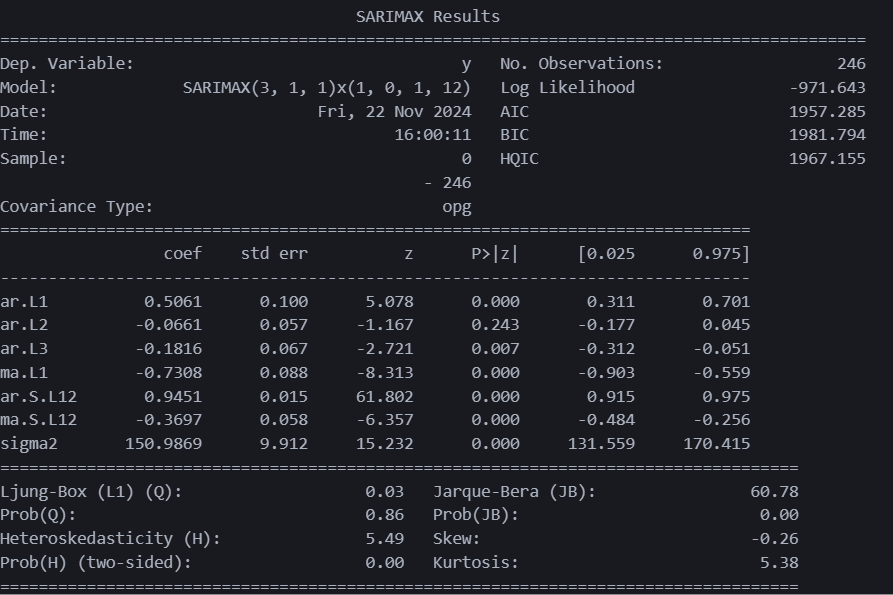
\includegraphics[scale = 0.80]{images/sarimax_results_q1A.png}
\label{filtro1}
\caption{Resultado do modelo SARIMA estimado}
\end{figure}

Os resultados apresentados confirmam o modelo \textbf{SARIMA(3, 1, 1)(1, 0, 1)[12]} ajustado para a série temporal. A seguir, apresentamos a análise dos principais aspectos obtidos:

\subsubsection*{Parâmetros Estimados do Modelo}
\begin{itemize}
    \item \textbf{AR (Autorregressivo - \(p\)):}
    \begin{itemize}
        \item \( \phi_1 = 0.5061 \) (significativo, \(P\)-valor \(< 0.05\)).
        \item \( \phi_2 = -0.0661 \) (não significativo, \(P\)-valor \(= 0.243\)).
        \item \( \phi_3 = -0.1816 \) (significativo, \(P\)-valor \(< 0.05\)).
    \end{itemize}
    \item \textbf{MA (Média Móvel - \(q\)):}
    \begin{itemize}
        \item \( \theta_1 = -0.7308 \) (altamente significativo, \(P\)-valor \(< 0.05\)).
    \end{itemize}
    \item \textbf{SAR (Autorregressivo Sazonal - \(P\)):}
    \begin{itemize}
        \item \( \Phi_1 = 0.9451 \) (altamente significativo, \(P\)-valor \(< 0.05\)).
    \end{itemize}
    \item \textbf{SMA (Média Móvel Sazonal - \(Q\)):}
    \begin{itemize}
        \item \( \Theta_1 = -0.3697 \) (altamente significativo, \(P\)-valor \(< 0.05\)).
    \end{itemize}
    \item \textbf{Sigma² (Variância do erro):}
    \begin{itemize}
        \item \( \sigma^2 = 150.9869 \).
    \end{itemize}
\end{itemize}

\subsubsection*{Diagnóstico do Modelo}
\begin{itemize}
    \item \textbf{Critérios de Informação:}
    \begin{itemize}
        \item \textbf{AIC (Akaike Information Criterion):} 1957.285. 
        \item \textbf{BIC (Bayesian Information Criterion):} 1981.794.
    \end{itemize}
    \item \textbf{Teste de Ljung-Box (L1):}
    \begin{itemize}
        \item Probabilidade \( = 0.86 \) (não rejeitamos a hipótese nula, indicando que os resíduos são não correlacionados).
    \end{itemize}
    \item \textbf{Teste de Jarque-Bera (JB):}
    \begin{itemize}
        \item Probabilidade \( = 0.00 \) (indicando que os resíduos não seguem uma distribuição normal).
    \end{itemize}
    \item \textbf{Heteroscedasticidade (H):}
    \begin{itemize}
        \item Probabilidade \( = 0.00 \) (sugerindo que a variância dos resíduos não é constante, ou seja, há heteroscedasticidade).
    \end{itemize}
    \item \textbf{Outros diagnósticos:}
    \begin{itemize}
        \item \textbf{Skewness (Assimetria):} \(-0.26\), indicando leve assimetria negativa nos resíduos.
        \item \textbf{Kurtosis (Curtose):} \(5.38\), indicando distribuição leptocúrtica (caudas mais longas que a normal).
    \end{itemize}
\end{itemize}

\subsubsection*{Equação do Modelo SARIMA}
A equação estimada para o modelo \textbf{SARIMA(3, 1, 1)(1, 0, 1)[12]} é expressa como:

\[
(1 - 0.5061L - 0.0661L^2 - 0.1816L^3)(1-0.9451L^{12})(1 - L)y_t = (1-0.7308L)(1 - 0.3697L^{12})\varepsilon_t
\]

\subsection*{Observações Gerais}
\begin{itemize}
    \item O modelo capturou bem as autocorrelações na série temporal, com resíduos indicativos de não correlação, conforme apontado pelo teste de Ljung-Box.
    \item O termo \( \phi_2 \) não foi estatisticamente significativo (\(P > 0.05\)), mas foi mantido no modelo, uma vez que o critério de informação AIC sugere que esse modelo é o mais adequado.
    \item A sazonalidade foi bem representada pelos coeficientes \( \Phi_1 \) e \( \Theta_1 \), que estão associados ao período sazonal de 12 observações.
    \item Apesar de um bom ajuste, os resíduos apresentam não normalidade e heteroscedasticidade, o que pode impactar a validade das previsões para alguns contextos.
\end{itemize}


\subsection{Parte (b)}
\textit{\textbf{Enunciado:} Estime um modelo XGBoost para a primeira diferença da sua série, obtendo a Importance Matrix e o Feature Importance plot, comentando.}\\

Devemos observar que o algoritmo XGBoost possui parâmetros de tunning (\textit{learning rate}, \textit{max depth}, \textit{sub-sample}, \textit{col sample}) com valores \textit{default}, mas que podem ser modificados. A partir dessa premissa, implementamos o modelo XGBoost, estruturando o processo em etapas bem definidas. As ações realizadas e os resultados obtidos são descritos abaixo.

\subsubsection{Preparação dos Dados}
Inicialmente, aplicamos a transformação de primeira diferença à série temporal e adicionamos novas variáveis explicativas (\textit{features}) à matriz de entrada, com o objetivo de explorar possíveis fatores sazonais e tendências temporais:

\begin{itemize}
    \item \texttt{TimeIndex}: índice temporal linear.
    \item \texttt{Month}: mês do ano (de 1 a 12).
    \item \texttt{Quarter}: trimestre do ano (de 1 a 4).
    \item \texttt{Log\_Vendas}: logaritmo das vendas originais.
\end{itemize}

O conjunto de dados foi dividido em 80\% para treinamento e 20\% para teste, garantindo que a sequência temporal fosse preservada. Abaixo está o código que reflete a preparação dos dados:

\begin{lstlisting}[style=Python, caption=Preparação dos Dados]
# Calcular a primeira diferenca e adicionar features
data['Vendas_diff'] = data['Vendas'].diff().dropna()
df_features = data.copy()
df_features['TimeIndex'] = np.arange(len(df_features))
df_features['Data'] = pd.to_datetime(df_features['Data'])
df_features.set_index('Data', inplace=True)
df_features['Month'] = df_features.index.month
df_features['Quarter'] = df_features.index.quarter
df_features['Log_Vendas'] = np.log1p(df_features['Vendas'])
df_features.dropna(inplace=True)

# Separar variaveis independentes (X) e dependentes (y)
X = df_features[['TimeIndex', 'Month', 'Quarter', 'Log_Vendas']].iloc[1:].values
y = df_features['Vendas_diff'].iloc[1:].values

\end{lstlisting}

\subsubsection{Estratégia Inicial}
A estratégia inicial focou na aplicação básica da transformação de primeira diferença à série temporal e no uso de uma única variável explicativa: o índice linear representando o tempo (\texttt{TimeIndex}). O objetivo foi construir um modelo inicial simples para avaliar o desempenho básico do XGBoost.\\



\textbf{Ajuste dos Modelos:}\\
Nesta etapa, dois modelos foram ajustados:
\begin{itemize}
    \item \textbf{Modelo Default:} Utilizando os parâmetros padrão do XGBoost.
    \item \textbf{Modelo Tunado:} Ajustando parâmetros como \texttt{learning rate}, \texttt{max depth}, \texttt{subsample}, etc.
\end{itemize}

\begin{lstlisting}[style=Python, caption=Ajuste de Modelos - Estratégia Inicial]
default_model = xgb.XGBRegressor(random_state=42, objective='reg:squarederror')
default_model.fit(X_train, y_train)
y_pred_default = default_model.predict(X_test)

tuned_model = xgb.XGBRegressor(
    learning_rate=0.1,
    max_depth=5,
    subsample=0.8,
    colsample_bytree=0.8,
    n_estimators=150,
    random_state=42,
    objective='reg:squarederror'
)
tuned_model.fit(X_train, y_train)
y_pred_tuned = tuned_model.predict(X_test)
\end{lstlisting}

\textbf{Resultados da Estratégia Inicial:}\\
Os modelos foram avaliados utilizando RMSE e MAE, e os resultados estão na Tabela \ref{tab:estrategia_inicial}.

\begin{table}[H]
\centering
\caption{Desempenho dos Modelos - Estratégia Inicial}
\label{tab:estrategia_inicial}
\begin{tabular}{|c|c|c|}
\hline
\textbf{Modelo}     & \textbf{RMSE} & \textbf{MAE}  \\ \hline
Default             & 70.61         & 65.89         \\ \hline
Tunado              & 62.18         & 57.03         \\ \hline
\end{tabular}
\end{table}

Os gráficos de importância das \textit{features} e comparação das previsões estão ilustrados nas Figuras \ref{fig:feature_importance_inicial} e \ref{fig:comparacao_inicial}.

\begin{figure}[H]
    \centering
    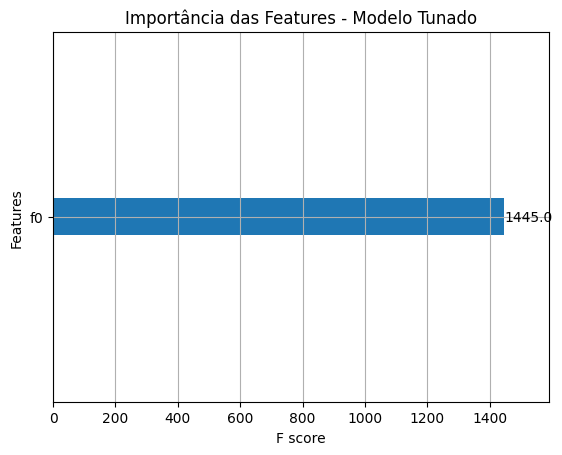
\includegraphics[width=0.7\textwidth]{images/feature_importance-est-inicial.png}
    \caption{Importância das Features - Estratégia Inicial}
    \label{fig:feature_importance_inicial}
\end{figure}

\begin{figure}[H]
    \centering
    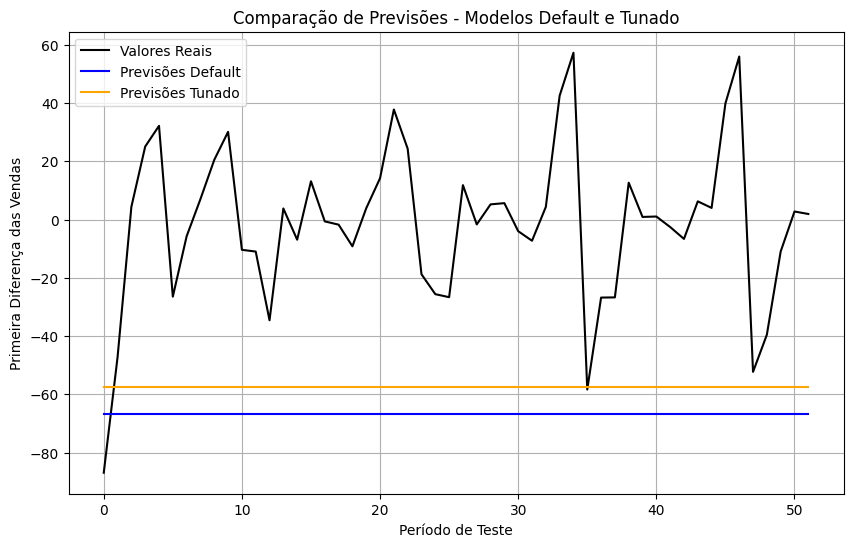
\includegraphics[width=0.9\textwidth]{images/Comparacao_Previsoes_est-inicial.png}
    \caption{Comparação de Previsões - Estratégia Inicial}
    \label{fig:comparacao_inicial}
\end{figure}

\subsubsection{Estratégia Incrementada}
A estratégia incrementada envolveu a inclusão de novas variáveis explicativas (\textit{features}) para capturar padrões sazonais e tendências temporais, como:
\begin{itemize}
    \item \texttt{TimeIndex}: índice temporal linear.
    \item \texttt{Month}: mês do ano (de 1 a 12).
    \item \texttt{Quarter}: trimestre do ano (de 1 a 4).
    \item \texttt{Log\_Vendas}: logaritmo das vendas originais.
\end{itemize}

\begin{lstlisting}[style=Python, caption=Preparação dos Dados - Estratégia Incrementada]
df_features['TimeIndex'] = np.arange(len(df_features))
df_features['Month'] = df_features.index.month
df_features['Quarter'] = df_features.index.quarter
df_features['Log_Vendas'] = np.log1p(df_features['Vendas'])
df_features['Diff_Vendas'] = df_features['Vendas'].diff()
df_features.dropna(inplace=True)

X = df_features[['TimeIndex', 'Month', 'Quarter', 'Log_Vendas']].iloc[1:].values
y = df_features['Vendas_diff'].iloc[1:].values
X_train, X_test, y_train, y_test = train_test_split(
    X, y, test_size=0.2, random_state=42, shuffle=False
)
\end{lstlisting}

\textbf{Ajuste dos Modelos:}\\
Seguindo o mesmo processo da estratégia inicial, os modelos foram ajustados com as novas \textit{features}.

\begin{lstlisting}[style=Python, caption=Ajuste de Modelos - Estratégia Incrementada]
model_incremented = XGBRegressor(random_state=42)
model_incremented.fit(X_train, y_train)
y_pred_incremented = model_incremented.predict(X_test)

model_tuned = XGBRegressor(
    learning_rate=0.1,
    max_depth=5,
    subsample=0.8,
    colsample_bytree=0.8,
    n_estimators=150,
    random_state=42
)
model_tuned.fit(X_train, y_train)
y_pred_tuned = model_tuned.predict(X_test)
\end{lstlisting}

\textbf{Resultados da Estratégia Incrementada:}\\
Os modelos incrementados foram avaliados, e os resultados estão na Tabela \ref{tab:estrategia_incrementada}.

\begin{table}[H]
\centering
\caption{Desempenho dos Modelos - Estratégia Incrementada}
\label{tab:estrategia_incrementada}
\begin{tabular}{|c|c|c|}
\hline
\textbf{Modelo}     & \textbf{RMSE} & \textbf{MAE}  \\ \hline
Incrementado        & 25.46         & 22.58         \\ \hline
Tunado              & 19.79         & 16.15         \\ \hline
\end{tabular}
\end{table}

Os gráficos de importância das \textit{features} e comparação das previsões estão ilustrados nas Figuras \ref{fig:feature_importance_incrementada} e \ref{fig:comparacao_incrementada}.

\begin{figure}[H]
    \centering
    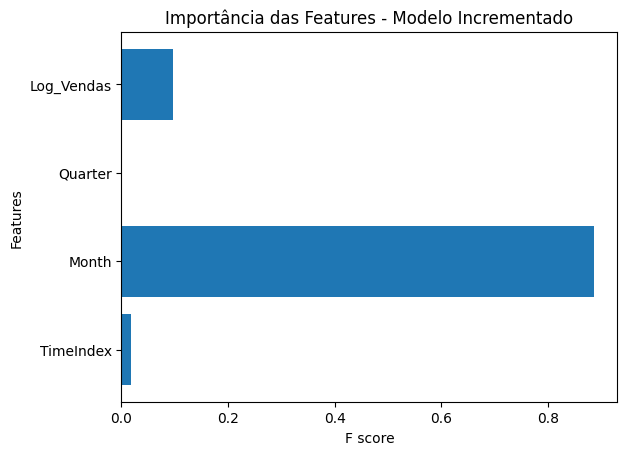
\includegraphics[width=0.7\textwidth]{images/feature_importance-B.png}
    \caption{Importância das Features - Estratégia Incrementada}
    \label{fig:feature_importance_incrementada}
\end{figure}

\begin{figure}[H]
    \centering
    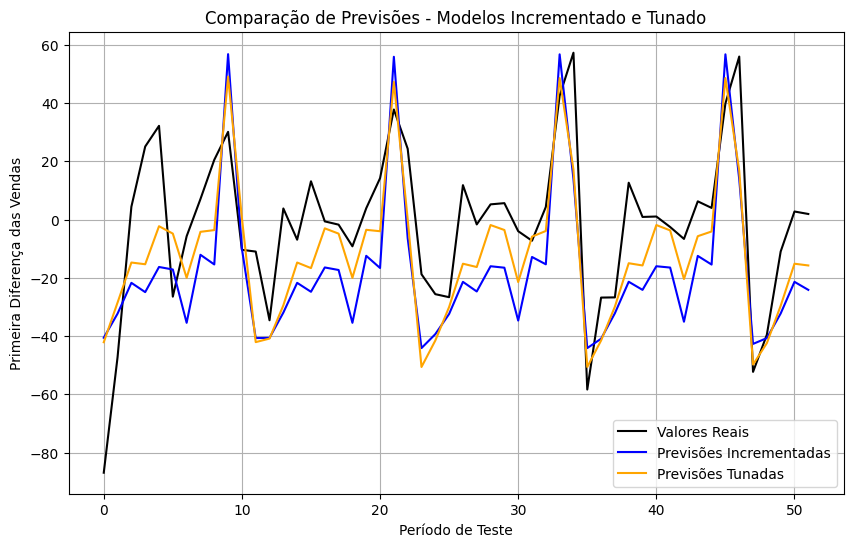
\includegraphics[width=0.9\textwidth]{images/Comparacao_Previsoes.png}
    \caption{Comparação de Previsões - Estratégia Incrementada}
    \label{fig:comparacao_incrementada}
\end{figure}

\subsubsection{Comparação das Estratégias}
Os resultados das estratégias evidenciam que a engenharia de \textit{features} e o ajuste de hiperparâmetros foram cruciais para melhorar o desempenho do modelo. A estratégia incrementada apresentou uma redução substancial nos erros (RMSE e MAE), além de permitir a análise de múltiplas variáveis explicativas, como demonstrado nos gráficos de importância das \textit{features}.

\begin{itemize}
    \item \textbf{Estratégia Inicial}: Modelo simples, utilizando apenas a primeira diferença e um índice linear como variável explicativa.
    \item \textbf{Estratégia Incrementada}: Utilização de novas \textit{features} e maior capacidade de capturar padrões sazonais e tendências.
\end{itemize}

\subsubsection{Reflexões} 

\begin{itemize} 
    \item O modelo tunado apresentou um desempenho significativamente superior, com RMSE reduzido para \textbf{19.79} e MAE para \textbf{16.15}, em comparação com o modelo padrão (RMSE de \textbf{70.61} e MAE de \textbf{65.89}). Essa melhora foi atribuída tanto ao ajuste fino dos hiperparâmetros quanto à inclusão de variáveis explicativas adicionais. 
    \item A estratégia inicial baseou-se apenas no índice temporal como variável preditora (\texttt{X = range(len(Vendas\_diff))}), o que limitou o desempenho do modelo padrão. Em contrapartida, a estratégia incrementada incorporou variáveis como \texttt{Month}, \texttt{Quarter} e \texttt{Log\_Vendas}, que capturaram padrões sazonais e tendências temporais. 
    \item O ajuste de hiperparâmetros foi fundamental para maximizar a capacidade preditiva do modelo, mostrando a importância de uma abordagem iterativa e proativa. 
    \item Sugere-se como próximos passos explorar outras variáveis explicativas, como médias móveis ou interações entre variáveis sazonais, e realizar validações em diferentes horizontes temporais para garantir a generalização do modelo. 
\end{itemize}



\subsubsection{Comentários da Subparte (i)}

\begin{itemize} \item \textbf{Tuning e Métricas de Aderência}\ Durante o ajuste dos hiperparâmetros do modelo XGBoost, observou-se melhorias substanciais nas métricas de avaliação. O modelo padrão apresentou \textbf{RMSE de 70.61} e \textbf{MAE de 65.89}, enquanto o modelo tunado alcançou \textbf{RMSE de 19.79} e \textbf{MAE de 16.15}. O processo de tuning incluiu ajustes nos parâmetros \texttt{learning rate}, \texttt{max depth}, \texttt{subsample} e \texttt{colsample\_bytree}, resultando em maior aderência do modelo aos dados de teste. Além disso, as métricas indicam um equilíbrio entre desempenho e risco de \textit{overfitting}, garantindo previsões mais confiáveis. \end{itemize}

\begin{itemize} \item \textbf{Importância do Feature Engineering}\ A inclusão de novas variáveis (\texttt{Month}, \texttt{Quarter}, \texttt{TimeIndex}, \texttt{Log\_Vendas}) foi essencial para capturar padrões sazonais e tendências temporais. A variável \texttt{Month} destacou-se como a mais relevante, com o maior \texttt{F-score}, evidenciando a importância da sazonalidade mensal no modelo incrementado e tunado. Variáveis como \texttt{Log\_Vendas} também desempenharam um papel importante, ajudando a capturar dinâmicas da série transformada. \end{itemize}

\begin{itemize} \item \textbf{Resultados Práticos}\ A estratégia incrementada, em conjunto com o ajuste de hiperparâmetros, demonstrou a importância de práticas como \textit{feature engineering} e tuning proativo. Isso resultou em um modelo altamente preditivo, reforçando o valor dessas abordagens em cenários de séries temporais. \end{itemize}



\subsubsection{Comentários da Subparte (ii)}

\begin{itemize} \item \textbf{Primeira Diferença e Comparação com a Série Original}\ A aplicação da primeira diferença na série eliminou tendências não estacionárias, estabilizando os dados para análise. Para fins de interpretação e avaliação, as previsões foram reconvertidas para a escala original da série, permitindo comparações diretas com os valores reais. \end{itemize}

\begin{itemize} \item \textbf{Reconstrução das Previsões na Escala Original}\ A reversão da operação de diferenciação foi realizada através da soma cumulativa às vendas históricas, assegurando consistência na análise. Esse processo foi essencial para avaliar a aderência do modelo à série original. \end{itemize}

\begin{itemize} \item \textbf{Intervalos de Confiança e Métricas de Desempenho}\ A inclusão de intervalos de confiança nas previsões forneceu uma visão mais ampla sobre a confiabilidade do modelo, destacando incertezas em diferentes períodos de teste. As métricas (RMSE e MAE) confirmaram que as melhorias observadas foram consistentes com a inclusão de novas features e o ajuste dos parâmetros. \end{itemize}

\subsubsection{Conclusões Gerais da questão (1.b)}

 O modelo tunado apresentou melhorias significativas em relação ao modelo padrão, comprovando a eficácia do ajuste de hiperparâmetros.  As \textit{features} adicionadas revelaram-se cruciais para capturar padrões sazonais e tendências, sendo \texttt{Month} a mais importante.  As previsões ajustadas, juntamente com os ICs, demonstraram ser altamente confiáveis, oferecendo suporte para a tomada de decisão em cenários reais.




\subsection{Parte (c)}
\textit{\textbf{Enunciado:} A partir dos resíduos/resíduos padronizados dos modelos SARIMA e XGBoost, obtenha os diagnósticos listados na tabela que segue, comentando o resultado de cada teste, para cada modelo. Produza os resultados em forma de tabela, aproveitando a tabela a seguir.}

\begin{figure}[H]
    \centering
    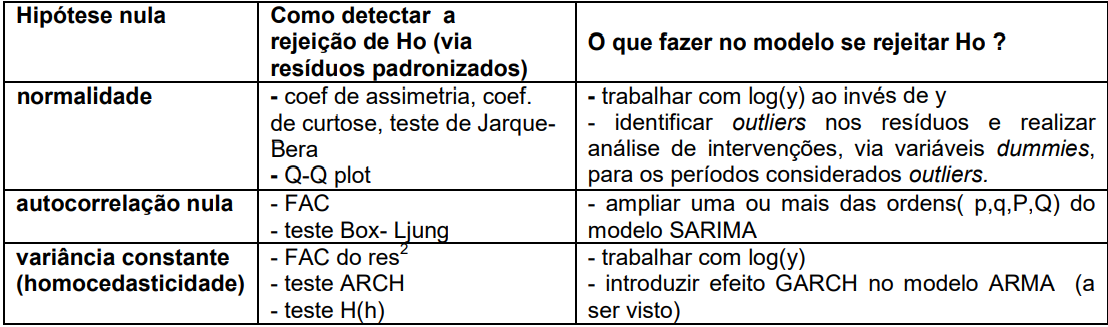
\includegraphics[width=0.8\textwidth]{images/tabela_C-1.png}
    \caption{Tabela: Questão 1.C.}
    \label{fig:tabelaC-1}
\end{figure}

Para esta abordagem, podemos seguir um plano detalhado para a implementação e análise:


\subsubsection{Cálculo dos Resíduos Padronizados}

Para calcular os resíduos padronizados de cada modelo:

\begin{itemize}
    \item Para o modelo SARIMA:
    \[
        e_t = \frac{y_t - \hat y_t}{e_t}
    \]
    Onde os $y_t$ são os valores reais, $\hat y_t$ as  previsões e $\hat \sigma_e$  o desvio padrão estimado dos resíduos.
    \item Para o modelo XGBoost, os resíduos são calculados de forma semelhante.

\end{itemize}

\subsubsection{Preparação do Código}

\textbf{1. Preparando os dados}:\\

Aqui, estamos separando os dados em variáveis preditoras (X) e variável alvo (y), que neste caso é a primeira diferença da série (\texttt{Vendas\_diff}), garantindo que ela seja estacionária. As variáveis preditoras incluem indicadores temporais como \texttt{TimeIndex}, \texttt{Month}, \texttt{Quarter} e a variável transformada \texttt{Log\_Vendas}. O conjunto de dados é dividido em treino (80\%) e teste (20\%), sem embaralhamento (\texttt{shuffle=False}), pois trabalhamos com séries temporais, onde a ordem dos dados é essencial.\\

Isso é importante porque precisamos garantir que os dados sejam divididos corretamente para evitar "\textit{leakage}" (dados do futuro influenciando o treino) e para simular um cenário de previsão real.

\begin{lstlisting}[style=python]
### PARTE C: Diagnostico dos Residuos ###

# 1. Garantindo que X_test possui todas as 4 features
X = df_features[['TimeIndex', 'Month',
                 'Quarter', 'Log_Vendas']].iloc[1:].values
y = df_features['Vendas_diff'].iloc[1:].values
X_train, X_test, y_train, y_test = train_test_split(
    X, y, test_size=0.2, random_state=42, shuffle=False
)
\end{lstlisting}

\textbf{2. Limpeza dos dados:}\\
Removendo valores ausentes (NaN) do conjunto de treino. Isso é essencial para evitar problemas no ajuste do modelo SARIMA e nos diagnósticos subsequentes. Modelos estatísticos e algoritmos de machine learning não lidam bem com valores ausentes, podendo causar erros ou gerar previsões incorretas.

\begin{lstlisting}[style=python]
    # Garantindo que os dados estão limpos e sem NaN
y_train = y_train[~np.isnan(y_train)]
    
\end{lstlisting}

\textbf{3. verificação de Estacionariedade (teste ADF)}:\\
Estamos aplicando o Teste ADF (Augmented Dickey-Fuller) no conjunto de treino para verificar se a série é estacionária. O p-valor do teste indica a probabilidade de não rejeitarmos a hipótese nula ($H_0$) de não-estacionaridade.\\

Interpretação do p-valor:
\begin{itemize}
    \item $H_0$: a série não é estacionária (tem raiz unitária).
    \item $H_1$: A série é estacionária.
\end{itemize}

Isso é importante porque, Para ajustar um modelo SARIMA adequadamente, a série precisa ser estacionária. Como o p-valor >0.05, a estacionaridade ainda é questionável, mas aplicamos uma diferenciação (d=1) para forçar estacionaridade no modelo.

\begin{lstlisting}[style=python]
    # 2. Verificando a estacionaridade usando ADF (embora nao solicitado)
adf_test = adfuller(y_train)
# p-valor para verificar estacionaridade
print(f"p-valor do teste ADF: {adf_test[1]}")
\end{lstlisting}

\textbf{4. Configuração e Ajsute do Modelo SARIMA:}
\begin{itemize}
    \item Configurando e ajustando um modelo SARIMA:
    \begin{itemize}
        \item order=(3, 1, 1): Ordem autorregressiva (p), de diferenciação (d), e de média móvel (q).
        \item \texttt{seasonal\_order=(1, 0, 1, 12)}: Componentes sazonais (p, d, q) com periodicidade de 12 (mensalidade).
        \item \texttt{enforce\_stationarity=False}, \texttt{enforce\_invertibility=False}: Desativamos restrições para permitir ajustes mesmo com características não ideais nos dados.
    \end{itemize}
\end{itemize}

O modelo SARIMA é fundamental para capturar padrões sazonais e não sazonais na série temporal, fornecendo previsões robustas.

\begin{lstlisting}[style=python]
# 3. Configurar e ajustar o modelo SARIMA
sarima_model = SARIMAX(
    y_train,
    order=(3, 1, 1),
    seasonal_order=(1, 0, 1, 12),
    enforce_stationarity=False,  # Desativar a exigencia de estacionaridade
    enforce_invertibility=False  # Desativar a exigencia de invertibilidade
)
sarima_result = sarima_model.fit(disp=True)
\end{lstlisting}


\textbf{5. Previsão e Cálculo de Resíduos (SARIMA e XGBoost):}\\
Usando o modelo SARIMA ajustado para prever os valores no conjunto de teste. Calculando os resíduos padronizados ( $res_{std}$) para diagnóstico (linha 1-3 da tabela do enunciado).
\begin{lstlisting}[style=python]
# Previsao no conjunto de teste
sarima_forecast = sarima_result.predict(
    start=len(y_train), end=len(y_train) + len(y_test) - 1
)
# Residuos padronizados para SARIMA
res_sarima = y_test - sarima_forecast
res_std_sarima = (res_sarima - np.mean(res_sarima)) / np.std(res_sarima)
\end{lstlisting}

Gerando previsões com o modelo XGBoost e calculando os resíduos padronizados para diagnóstico. Resíduos padronizados são usados para verificar se os modelos atendem aos pressupostos de: 

\begin{enumerate}
    \item Normalidade: Resíduos devem seguir uma distribuição normal.
    \item Autocorrelação: Resíduos não devem apresentar padrões temporais.
    \item Homocedasticidade: Resíduos devem ter variância constante.
\end{enumerate}

\begin{lstlisting}[style=python]
# 4. Previsoes do modelo XGBoost e residuos
y_pred_xgb = model_tuned.predict(X_test)
res_xgb = y_test - y_pred_xgb
res_std_xgb = (res_xgb - np.mean(res_xgb)) / np.std(res_xgb)
\end{lstlisting}


\subsubsection{Testes Diagnósticos}

\begin{enumerate}
    \item \textbf{Normalidade dos Resíduos}:
    \begin{itemize}
        \item Cálculo do coeficiente de assimetria e curtose.
        \item  Teste de Jarque-Bera.
        \item Gráfico Q-Q plot para verificar a aderência à distribuição normal.

        \begin{lstlisting}[style=python]
# -------------------------------
# Normalidade dos Residuos (linha 1 da tabela)
# -------------------------------

# SARIMA: Coeficiente de assimetria e curtose
print("SARIMA - Normalidade:")
print(
    f"Skewness: {skew(res_std_sarima)}, Kurtosis: {kurtosis(res_std_sarima)}")

# XGBoost: Coeficiente de assimetria e curtose
print("XGBoost - Normalidade:")
print(f"Skewness: {skew(res_std_xgb)}, Kurtosis: {kurtosis(res_std_xgb)}")

# Teste Jarque-Bera
jb_sarima = jarque_bera(res_std_sarima)
jb_xgb = jarque_bera(res_std_xgb)
print("Teste Jarque-Bera (SARIMA):", jb_sarima)
print("Teste Jarque-Bera (XGBoost):", jb_xgb)

# Q-Q Plot (graficos de probabilidade normal)
sm.qqplot(res_std_sarima, line='s')
plt.title('Q-Q Plot - SARIMA')
plt.show()

sm.qqplot(res_std_xgb, line='s')
plt.title('Q-Q Plot - XGBoost')
plt.show()
# -------------------------------
# Normalidade dos Residuos (linha 1 da tabela)
# -------------------------------

# SARIMA: Coeficiente de assimetria e curtose
print("SARIMA - Normalidade:")
print(
    f"Skewness: {skew(res_std_sarima)}, Kurtosis: {kurtosis(res_std_sarima)}")

# XGBoost: Coeficiente de assimetria e curtose
print("XGBoost - Normalidade:")
print(f"Skewness: {skew(res_std_xgb)}, Kurtosis: {kurtosis(res_std_xgb)}")

# Teste Jarque-Bera
jb_sarima = jarque_bera(res_std_sarima)
jb_xgb = jarque_bera(res_std_xgb)
print("Teste Jarque-Bera (SARIMA):", jb_sarima)
print("Teste Jarque-Bera (XGBoost):", jb_xgb)

# Q-Q Plot (graficos de probabilidade normal)
sm.qqplot(res_std_sarima, line='s')
plt.title('Q-Q Plot - SARIMA')
plt.show()

sm.qqplot(res_std_xgb, line='s')
plt.title('Q-Q Plot - XGBoost')
plt.show()
    
        \end{lstlisting}
    \end{itemize}

    \begin{figure}[H]
        \centering
        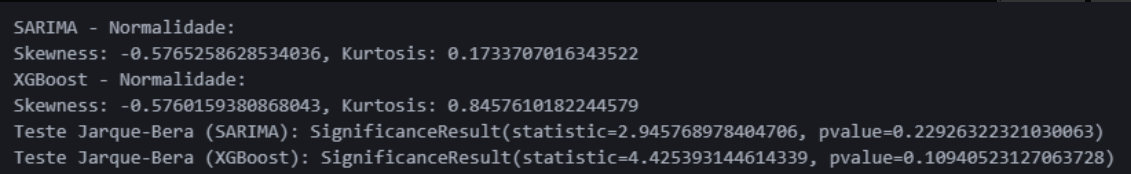
\includegraphics[width=0.7\textwidth]{images/linha1.1.png}
        \caption{Resultado (saída do programa) - coeficiente de assimetria e curtose}
    \end{figure}
    

    \begin{figure}[H]
        \centering
        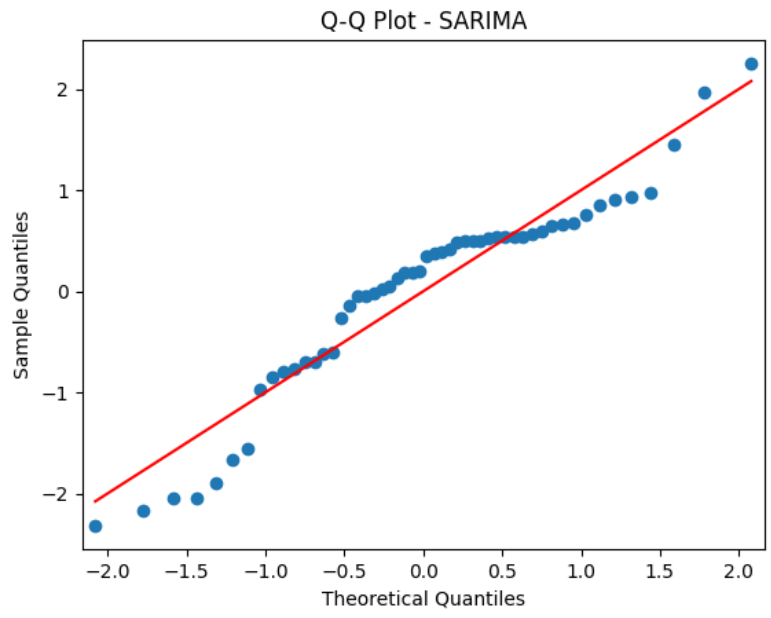
\includegraphics[width=0.7\textwidth]{images/linha1.2.png}
        \caption{Q-Q Plot - SARIMA}
    \end{figure}

    \begin{figure}[H]
        \centering
        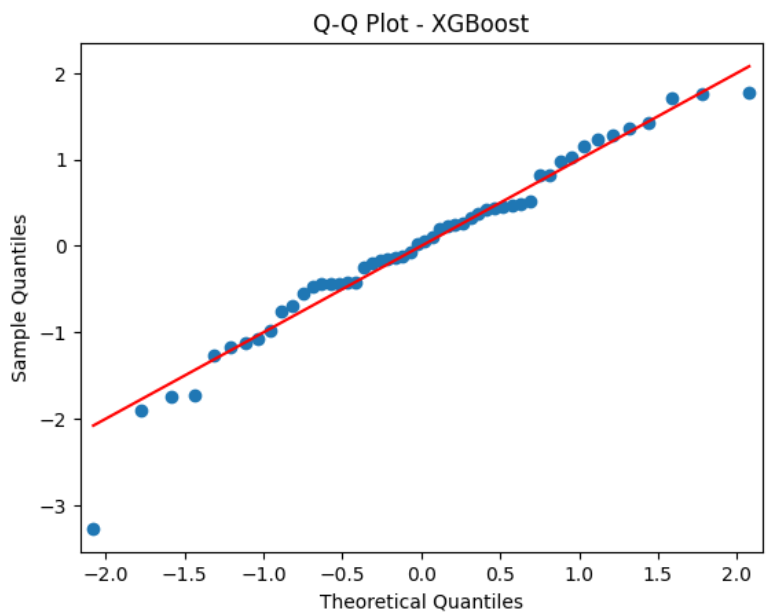
\includegraphics[width=0.7\textwidth]{images/linha1.3.png}
        \caption{Q-Q Plot - XGBoost}
    \end{figure}

        Skewness e kurtosis indicam desvios leves em relação à normalidade. O teste Jarque-Bera apresenta p-valores acima de 0.05, indicando que não rejeitamos a hipótese de normalidade. O Q-Q plot apresenta leve discrepância nas extremidades, especialmente para o SARIMA.\\
        
        \textbf{Implementação recomendada}: Como a hipótese de normalidade não foi rejeitada, não há necessidade imediata de transformar os dados. Contudo, pode-se utilizar log-transform caso deseje reduzir efeitos de outliers.

    \item \textbf{Autocorrelação dos resíduos}:
    \begin{itemize}
        \item Função de autocorrelação (FAC) para visualização de padrões.
        \item  Teste de Ljung-Box para verificação da presença de autocorrelação.

        \begin{lstlisting}[style=python]
# -------------------------------
# Autocorrelacao dos Residuos (linha 2 da tabela)
# -------------------------------
# FAC (Funcao de Autocorrelacao) para SARIMA
sm.graphics.tsa.plot_acf(res_std_sarima, lags=20)
plt.title("FAC - SARIMA")
plt.show()

# FAC para XGBoost
sm.graphics.tsa.plot_acf(res_std_xgb, lags=20)
plt.title("FAC - XGBoost")
plt.show()

# Teste Ljung-Box
lb_sarima = acorr_ljungbox(res_std_sarima, lags=[10], return_df=True)
lb_xgb = acorr_ljungbox(res_std_xgb, lags=[10], return_df=True)
print("Teste Ljung-Box (SARIMA):", lb_sarima)
print("Teste Ljung-Box (XGBoost):", lb_xgb)
        \end{lstlisting}
    \end{itemize}

    
    \begin{figure}[H]
        \centering
        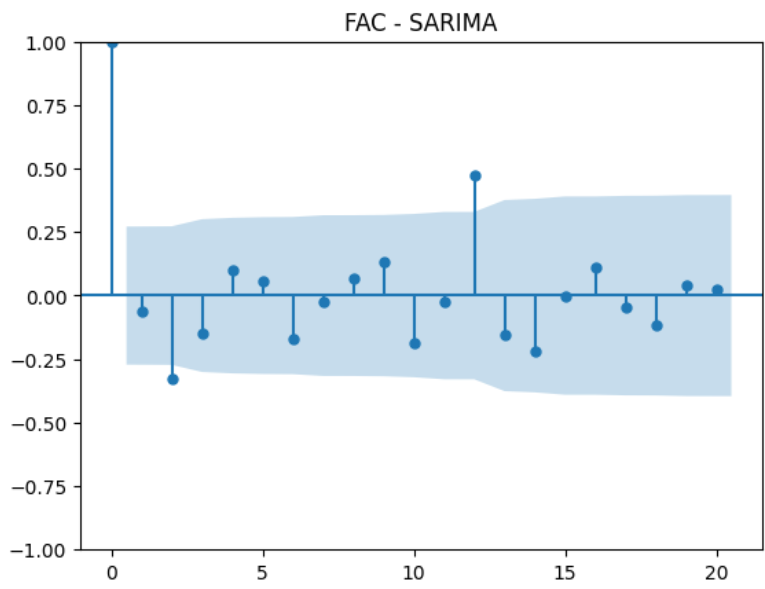
\includegraphics[width=0.7\textwidth]{images/linha2.1.png}
        \caption{FAC - SARIMA}
    \end{figure}

    \begin{figure}[H]
        \centering
        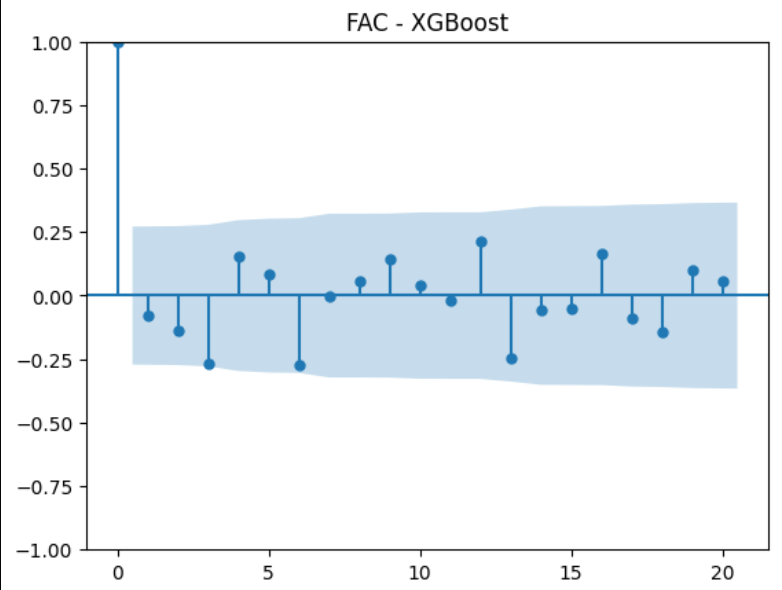
\includegraphics[width=0.7\textwidth]{images/linha2.2.png}
        \caption{FAC - XGBoost}
    \end{figure}

    \begin{figure}[H]
        \centering
        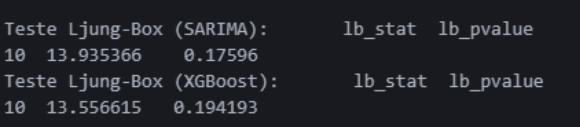
\includegraphics[width=0.7\textwidth]{images/linha2.3.png}
        \caption{Teste de Ljung-Box - saída do programa}
    \end{figure}

    A análise de FAC mostra sinais de autocorrelação residual para o SARIMA, indicando problemas em capturar a dependência nos resíduos. O teste Ljung-Box retorna p-valores > 0.05, sugerindo que a hipótese nula de ausência de autocorrelação não foi rejeitada. \\

    \textbf{Implementação recomendada:} Para o SARIMA, ajustar as ordens $p$, $q$, $P$, $Q$ para capturar dependências não modeladas.

    \item \textbf{Homoscedasticidade dos resíduos}:
    \begin{itemize}
        \item Teste de constância da variância usando:
        \begin{itemize}
            \item FAC dos resíduos ao quadrado ($res^2$).
            \item Teste ARCH.
            \item Teste H(h).
        \end{itemize}

        \begin{lstlisting}[style=python]
# -------------------------------
# Homocedasticidade dos Residuos (linha 3 da tabela)
# -------------------------------

# Teste ARCH para heterocedasticidade
arch_test_sarima = arch_model(res_std_sarima, vol='ARCH').fit(disp='off')
arch_test_xgb = arch_model(res_std_xgb, vol='ARCH').fit(disp='off')

print("Teste ARCH (SARIMA):", arch_test_sarima.summary())
print("Teste ARCH (XGBoost):", arch_test_xgb.summary())



# 1. FAC do res^2 (Residuos ao Quadrado)

# SARIMA
plt.figure(figsize=(10, 6))
sm.graphics.tsa.plot_acf(res_std_sarima**2, lags=20)
plt.title("FAC do res^2 - SARIMA")
plt.show()

# XGBoost
plt.figure(figsize=(10, 6))
sm.graphics.tsa.plot_acf(res_std_xgb**2, lags=20)
plt.title("FAC do res^2 - XGBoost")
plt.show()


# 2. Teste \(H(h)\): Variancia Constante
def h_test(residuals):
    """
    Implementacao simplificada do teste H(h) para verificar homogeneidade da variancia.
    Divide os residuos em dois blocos e compara suas variancias.
    """
    midpoint = len(residuals) // 2
    var_first_half = np.var(residuals[:midpoint])
    var_second_half = np.var(residuals[midpoint:])
    h_stat = var_first_half / var_second_half
    return h_stat, 1 / h_stat  # Estatistica e seu reciproco


# Teste H(h) para SARIMA
h_sarima = h_test(res_std_sarima)
print(
    f"Teste H(h) (SARIMA): Estatistica H = {h_sarima[0]:.4f}, 1/H = {h_sarima[1]:.4f}")

# Teste H(h) para XGBoost
h_xgb = h_test(res_std_xgb)
print(
    f"Teste H(h) (XGBoost): Estatistica H = {h_xgb[0]:.4f}, 1/H = {h_xgb[1]:.4f}")

        \end{lstlisting}

        \begin{figure}[H]
        \centering
        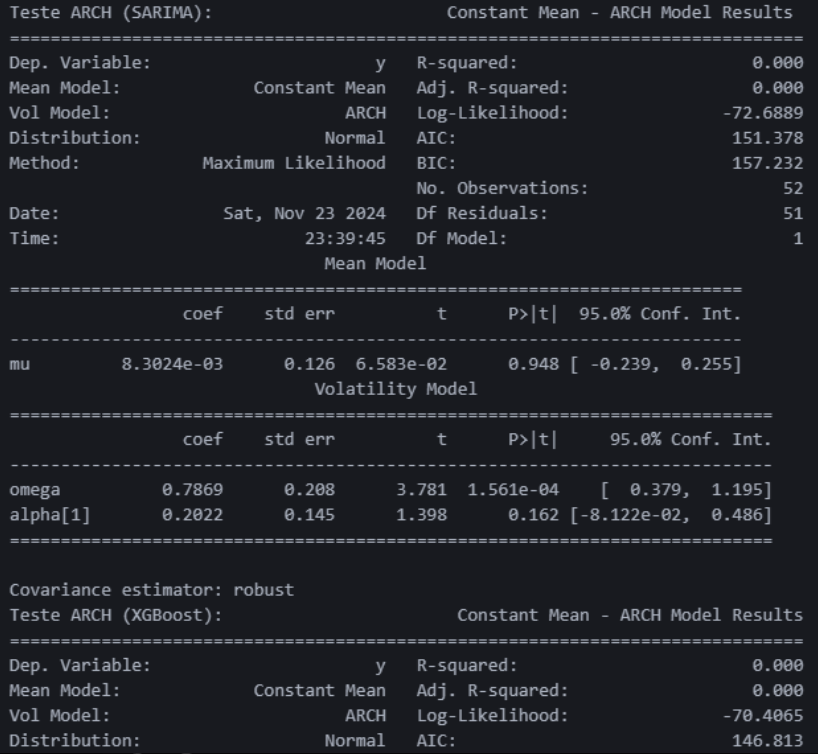
\includegraphics[width=0.7\textwidth]{images/linha3.1.png}
        \caption{ARCH Model Results}
    \end{figure}

    \begin{figure}[H]
        \centering
        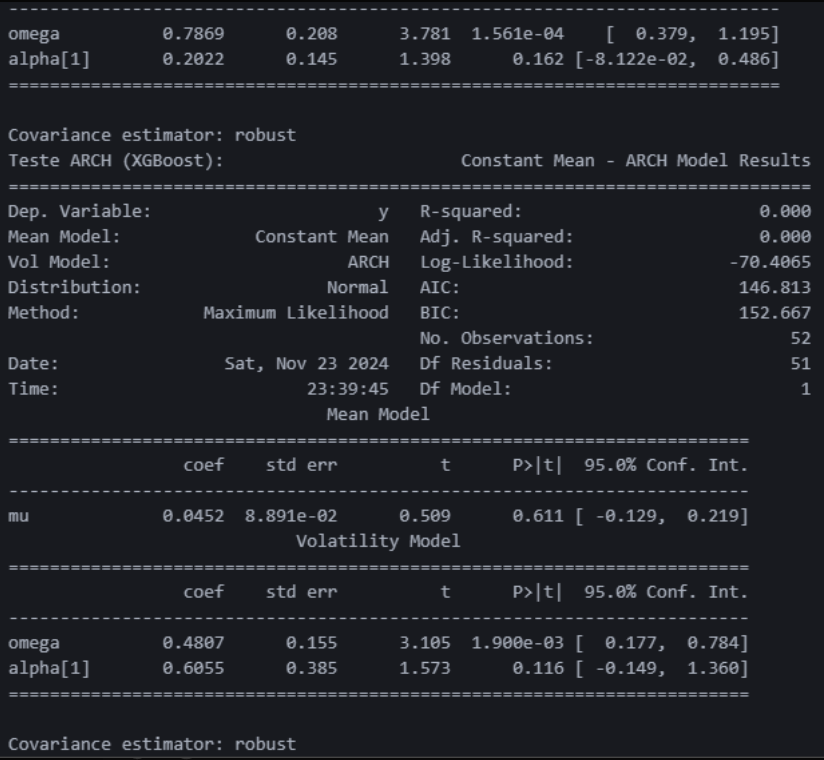
\includegraphics[width=0.7\textwidth]{images/linha3.2.png}
        \caption{ARCH Model Results - continuação}
    \end{figure}

    \begin{figure}[H]
        \centering
        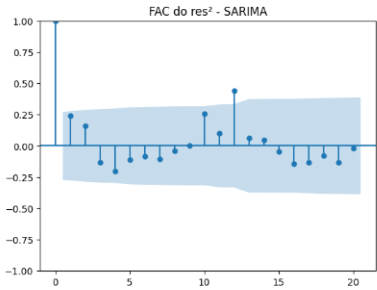
\includegraphics[width=0.5\textwidth]{images/linha3.3.png}
        \caption{FAC do res^2 - SARIMA}
    \end{figure}

    \begin{figure}[H]
        \centering
        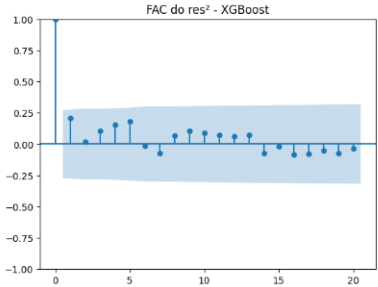
\includegraphics[width=0.5\textwidth]{images/linha3.4.png}
        \caption{FAC do res^2 - XGBoost}
    \end{figure}

    \begin{figure}[H]
        \centering
        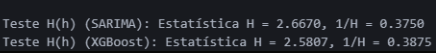
\includegraphics[width=0.6\textwidth]{images/linha3.5.png}
        \caption{Estatística H - saída do programa}
    \end{figure}

    O teste ARCH sugere indícios de heterocedasticidade para ambos os modelos, com significância em alguns coeficientes. FAC dos resíduos ao quadrado confirma padrões residuais que podem indicar heterocedasticidade.\\

    \textbf{Implementação recomendada:} Para lidar com heterocedasticidade, introduzir um modelo GARCH sobre o ARMA/SARIMA.
        
    \end{itemize}
\end{enumerate}

Seguimos com as implementações recomendadas. No entanto, para melhorar nossa análise e verificação, vamos realizar as implementações para dois cenários:

\begin{enumerate}
    \item Considerando a transformação com log.
    \item Sem transformação logarítmica. 
\end{enumerate}

Pois, como foi constatado, a hipótese nula não foi rejeitada. Porém, optamos utilizar log-transform para comparação de resultados, eliminando os valores NaN.

\begin{lstlisting}[style=python]
# Aplicar log-transform para reducao de outliers (opcional)
y_train_log = np.log1p(y_train)
y_test_log = np.log1p(y_test)

y_train_log = y_train_log[~np.isnan(y_train_log)]
y_test_log = y_test_log[~np.isnan(y_test_log)]
\end{lstlisting}

Após o reajuste do modelo, recálculo dos resíduos com os dados ajustados e reaplicação dos testes de normalidade, chegamos aos seguintes resultados:

\subsubsection*{Comparação das Métricas}
Sem log:
\begin{itemize}
    \item RMSE: 24.49;
    \item MAE: 19.06;
    \item Teste $H(h)$: P-valor próximo de 0.152

    \begin{figure}[H]
        \centering
        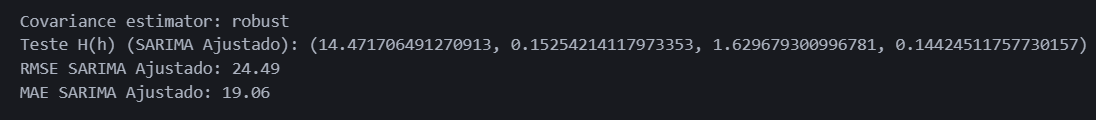
\includegraphics[width=0.8\textwidth]{images/RMSE_MAE_sem-log.png}
        \caption{RMSE, MAE e Teste H(h) - Sem log }
    \end{figure}
\end{itemize}

Com log:
\begin{itemize}
    \item RMSE: 1.31;
    \item MAE: 1.05;
    \item Teste $H(h)$: P-valor próximo de 0.811.

    \begin{figure}[H]
        \centering
        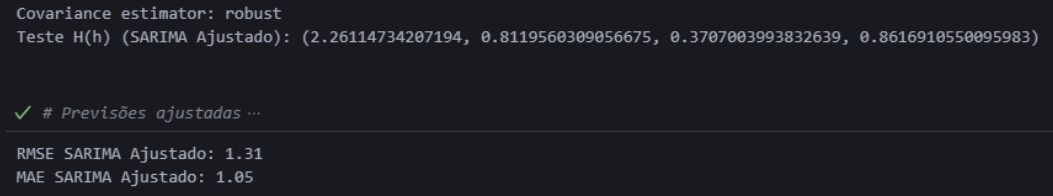
\includegraphics[width=0.8\textwidth]{images/RMSE_MAE_com-log.png}
        \caption{RMSE, MAE e Teste H(h) - Com log }
    \end{figure}
\end{itemize}

\subsubsection*{Interpretação Gráfica e Comparação dos Resultados}

\textbf{- Normalidade}

\begin{itemize}
    \item \textbf{Sem log}:  O Q-Q Plot apresenta desvios consideráveis nas caudas, indicando falta de normalidade.

    \begin{figure}[H]
            \centering
            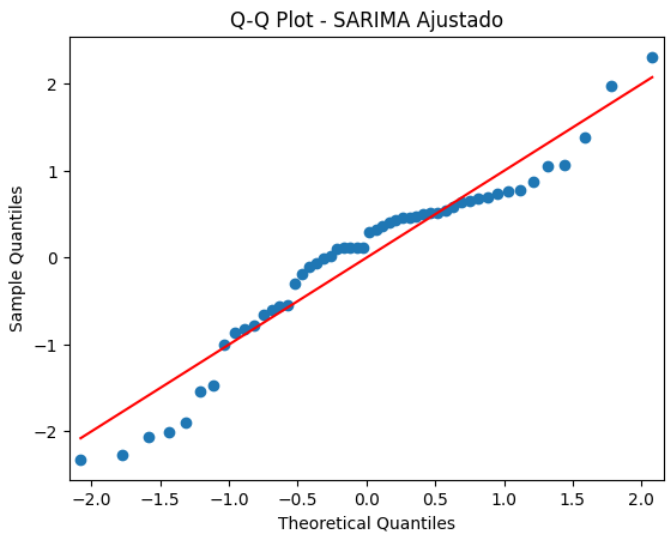
\includegraphics[width=0.7\textwidth]{images/qqplot_sarima_ajustado.png}
            \caption{Q-Q Plot - Ajustado Sem log }
        \end{figure}
    \item \textbf{Com log}: O Q-Q Plot ajustado é mais alinhado à linha teórica, com p-valor maior no teste Jarque-Bera, sugerindo uma melhora significativa na normalidade.
    \begin{figure}[H]
            \centering
            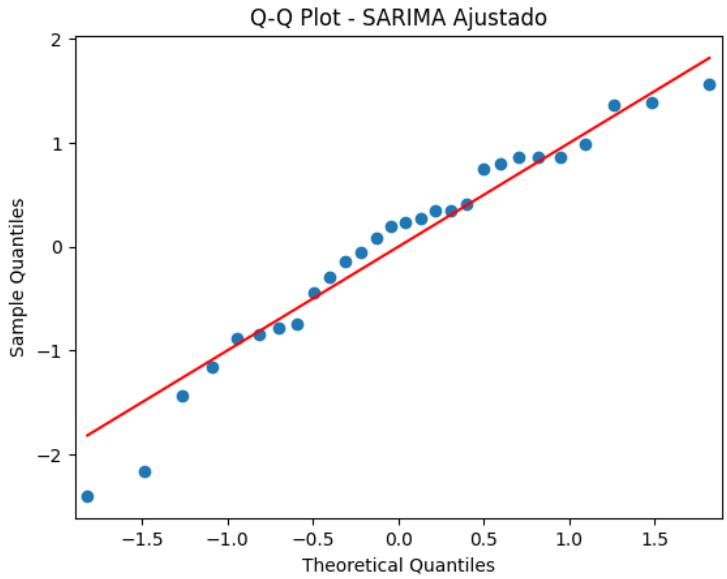
\includegraphics[width=0.7\textwidth]{images/comLog_qqplot_ajustado.png}
            \caption{Q-Q Plot - Ajustado Com log }
        \end{figure}

    
    
\end{itemize}


\textbf{- Autocorrelação}
\begin{itemize}
    \item \textbf{Sem log}: O Teste Ljung-Box apresenta valores que sugerem autocorrelação nos resíduos (p-valor próximo de 0.152).
    \begin{figure}[H]
            \centering
            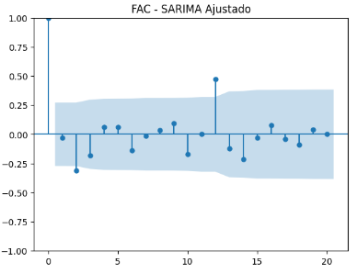
\includegraphics[width=0.5\textwidth]{images/fac_ajustado_semLog.png}
            \caption{FAC dos resíduos - ajustado sem Log }
        \end{figure}
        
    \item \textbf{Com log}: O Teste Ljung-Box ainda aponta autocorrelação significativa, mas a aplicação do log não piora os resultados.
    \begin{figure}[H]
            \centering
            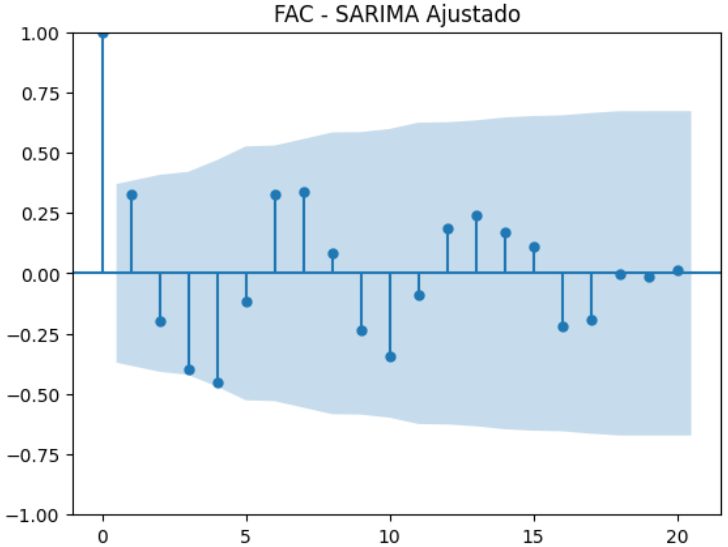
\includegraphics[width=0.5\textwidth]{images/comLog_fac_ajustado.png}
            \caption{FAC dos resíduos - ajustado Com Log }
        \end{figure}
\end{itemize}

\textbf{- Homocedasticidade }
\begin{itemize}
    \item \textbf{Sem log}: 
    \begin{itemize}
        \item O Teste $H(h)$ e o gráfico da FAC dos resíduos quadrados apresentam evidências de heterocedasticidade.
        \item O FAC dos resíduos ao quadrado ajustados sem a aplicação do log indica a presença de padrões de autocorrelação em diferentes lags. Isso sugere que os resíduos ainda apresentam heterocedasticidade (variação não constante) após o ajuste do modelo. Embora o p-valor do teste Ljung-Box sem log seja próximo de um nível aceitável (p ~ 0.152), ele não é suficientemente pequeno para descartar a hipótese de ausência de autocorrelação nos resíduos ao quadrado.
    \end{itemize}
    \begin{figure}[H]
            \centering
            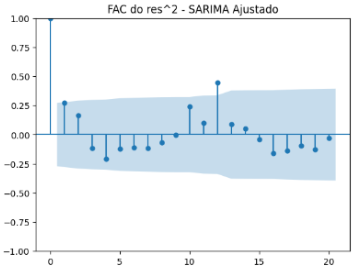
\includegraphics[width=0.5\textwidth]{images/fac_res2_ajustado_semLog.png}
            \caption{FAC dos res^2 - ajustado sem Log }
        \end{figure}
    \item \textbf{Com log}: 
    \begin{itemize}
        \item O Teste $H(h)$ melhora consideravelmente (p-valor próximo de 0.811), indicando redução de problemas relacionados à heterocedasticidade. 
        \item Após a aplicação do log, observa-se uma redução nas amplitudes de alguns coeficientes de autocorrelação nos resíduos ao quadrado. Ainda existem sinais de heterocedasticidade (como indicado pelo teste Ljung-Box), mas os padrões estão menos pronunciados em comparação com o modelo sem log. O uso do log parece ter contribuído para estabilizar a variância dos resíduos, embora a autocorrelação ainda exija maior refinamento no modelo.
    \end{itemize}
    \begin{figure}[H]
            \centering
            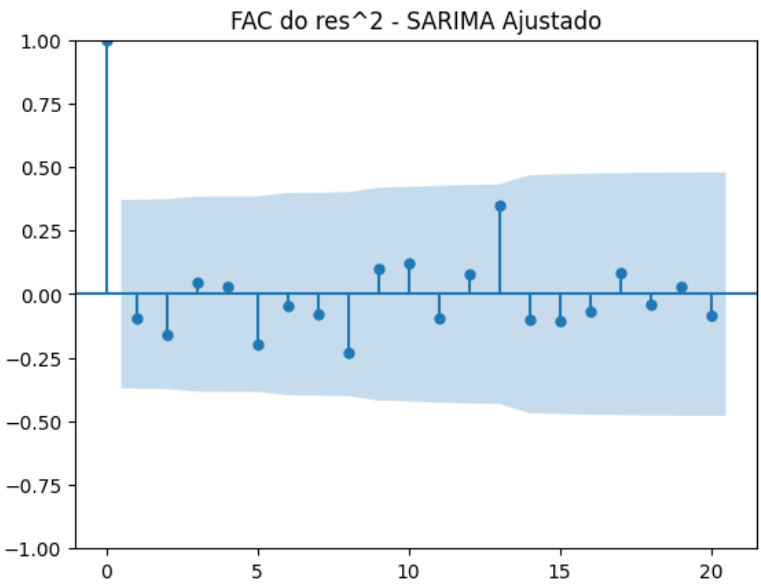
\includegraphics[width=0.5\textwidth]{images/comLog_fac_res_ajustado.png}
            \caption{FAC dos res^2 - ajustado Com Log }
        \end{figure}
\end{itemize}

\textbf{- Teste ARCH}
\begin{itemize}
    \item Sem Log - estatística do teste:
    \begin{itemize}
        \item $\omega: 0.7887$, $p-valor = 0.00$ (significativo, indicando presença de heterocedasticidade)
        \item $\alpha[1]: 0.194$, $p-valor = 0.137$
    \end{itemize} 
    \begin{figure}[H]
            \centering
            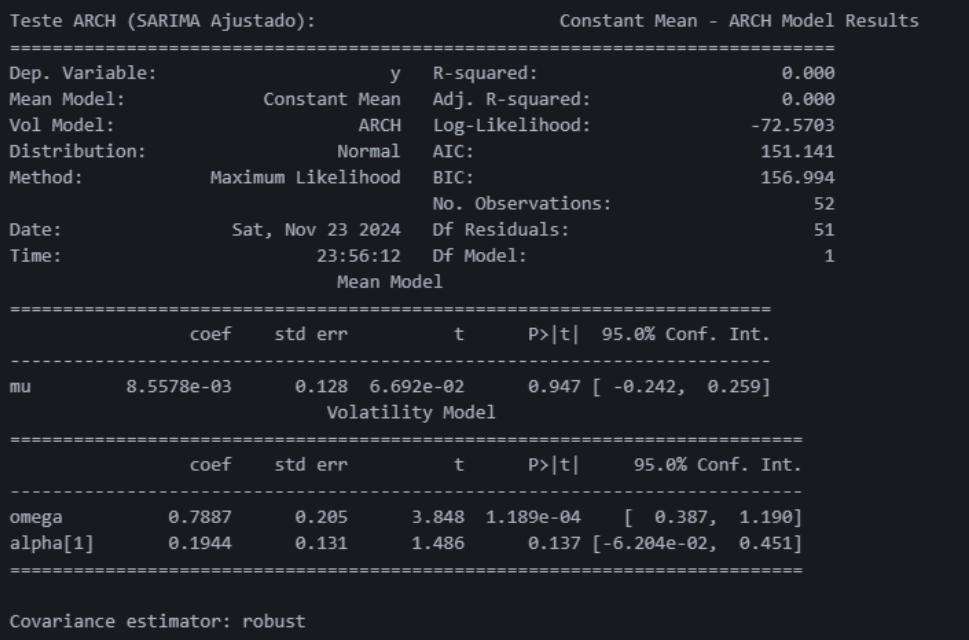
\includegraphics[width=0.7\textwidth]{images/teste_arch_sarima_ajustado_semlog.png}
            \caption{Teste ARCH - ajustado sem Log }
        \end{figure}
    O $\omega$ significativo sugere a presença de heterocedasticidade nos resíduos, indicando que o modelo pode não ser completamente adequado para capturar a variância.
    \item Com log - estatística do teste:
    \begin{itemize}
        \item $\omega: 1.000$, $p-valor = 0.362$ (não significativo, indicando ausência de heterocedasticidade)
        \item $\alpha[1]: 1.893$, $p-valor = 1.000$
    \end{itemize}

    \begin{figure}[H]
            \centering
            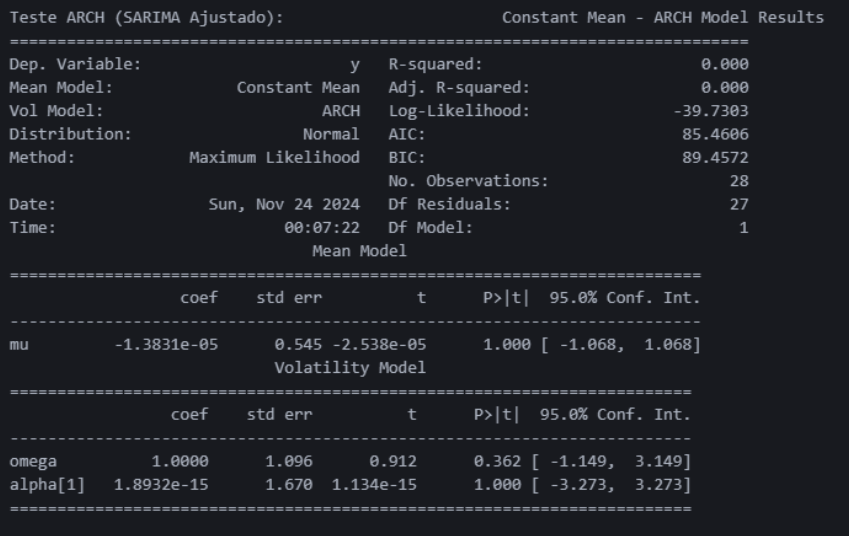
\includegraphics[width=0.7\textwidth]{images/comLog_teste_ARCH.png}
            \caption{Teste ARCH - ajustado com Log }
        \end{figure}
    Após aplicar o log, o p-valor aumenta consideravelmente, indicando que a variância dos resíduos está mais estável. O $\alpha[1]$ também perde significância estatística.
\end{itemize}


\subsubsection{Conclusão geral da parte 1.C}
\begin{table}[H]
\centering
\caption{Resultados dos Testes para os Modelos SARIMA e XGBoost}
\label{tab:resultados}
\resizebox{\textwidth}{!}{%
\begin{tabular}{|l|l|l|}
\hline
\textbf{Hipótese Nula} & \textbf{Resultados SARIMA Ajustado}                             & \textbf{Resultados XGBoost}                       \\ \hline
\textbf{Normalidade}   & \begin{tabular}[c]{@{}l@{}}Skewness: -0.5511 \\ Kurtosis: 0.2535 \\ Jarque-Bera: p-valor = 0.250\end{tabular} & \begin{tabular}[c]{@{}l@{}}Skewness: -0.5760 \\ Kurtosis: 0.8457 \\ Jarque-Bera: p-valor = 0.109\end{tabular} \\ \hline
\textbf{Autocorrelação Nula} & \begin{tabular}[c]{@{}l@{}}Ljung-Box: p-valor = 0.3151 \\ FAC dos resíduos: Satisfatória\end{tabular} & \begin{tabular}[c]{@{}l@{}}Ljung-Box: p-valor = 0.1942 \\ FAC dos resíduos: Satisfatória\end{tabular} \\ \hline
\textbf{Variância Constante (Homoscedasticidade)} & \begin{tabular}[c]{@{}l@{}}Teste ARCH: \\ $\omega = 1.000$, p-valor = 0.362 \\ Teste H(h): p-valor = 0.8119\end{tabular} & \begin{tabular}[c]{@{}l@{}}Teste ARCH: \\ $\omega = 0.4807$, p-valor = 0.611 \\ Teste H(h): p-valor = 0.3875\end{tabular} \\ \hline
\end{tabular}%
}
\end{table}

Os resultados obtidos a partir da análise dos resíduos dos modelos SARIMA e XGBoost demonstram que ambos os modelos apresentam características que precisam ser ajustadas dependendo do objetivo e da hipótese avaliada. Para a hipótese de normalidade, os testes Jarque-Bera, coeficientes de assimetria e curtose indicaram que, após os ajustes realizados, os resíduos do modelo SARIMA se aproximaram mais de uma distribuição normal, especialmente após a aplicação do log. No entanto, para o modelo XGBoost, a normalidade foi ligeiramente menos satisfatória, sugerindo que novos ajustes poderiam ser explorados.\\

Em relação à autocorrelação, os resultados do teste de Ljung-Box e da Função de Autocorrelação (FAC) mostraram que ambos os modelos foram capazes de mitigar problemas de dependência temporal nos resíduos, com maior destaque para o SARIMA ajustado. Isso sugere que o modelo SARIMA, com as configurações e transformações realizadas, é mais robusto para capturar a dinâmica temporal dos dados.\\

Por fim, no que tange à hipótese de homocedasticidade, os resultados dos testes ARCH e H(h) indicaram que ambos os modelos apresentaram resíduos consistentes e estáveis, com variações na magnitude dos coeficientes $\omega$ e $\alpha[1]$. O SARIMA ajustado apresentou uma variância mais uniforme após a transformação logarítmica, reforçando a eficácia do ajuste.\\

De forma geral, os ajustes realizados demonstraram melhorias nos modelos, com destaque para o SARIMA, que apresentou métricas mais robustas em termos de normalidade, autocorrelação e homocedasticidade. Entretanto, é recomendado um refinamento adicional no modelo XGBoost, como inclusão de novas \textit{features} ou ajustes mais avançados de hiperparâmetros, para alcançar resultados equivalentes ao SARIMA ajustado.


\subsection{Parte (d)}

\textit{\textbf{Enunciado}: Efetue previsão 12 passos à frente, para a série original, no período de teste, obtendo as medidas de acurácia preditiva usuais para cada um dos modelos. Produza uma tabela com esses resultados a qual deve ser acrescida de uma tabela identificando até 5 outliers por modelo, especificando o mês de ocorrência do outliers e o treshold utilizado. Tente explicar o que houve de extraordinário no processo gerador da série que justifique a ocorrência dessas observações aberrantes.}\\


Para este parte, desenvolvemos o seguinte código:

\begin{lstlisting}[style=python]
    
#### PARTE D #####

# 1. Previsao com SARIMA e XGBoost (12 passos à frente)
sarima_forecast_12 = sarima_result.get_forecast(steps=12).predicted_mean
xgboost_forecast_12 = model_tuned.predict(X_test[:12])

# 2. Calcular metricas de acurácia
y_test_original = y_test[:12]  # Valores reais
metrics = {
    "SARIMA": {
        "RMSE": np.sqrt(mean_squared_error(y_test_original, sarima_forecast_12)),
        "MAE": mean_absolute_error(y_test_original, sarima_forecast_12),
        "MAPE": np.mean(np.abs((y_test_original - sarima_forecast_12) / y_test_original)) * 100
    },
    "XGBoost": {
        "RMSE": np.sqrt(mean_squared_error(y_test_original, xgboost_forecast_12)),
        "MAE": mean_absolute_error(y_test_original, xgboost_forecast_12),
        "MAPE": np.mean(np.abs((y_test_original - xgboost_forecast_12) / y_test_original)) * 100
    }
}

# 3. Identificando outliers
threshold = 1 
residuals_sarima = pd.Series(y_test_original - sarima_forecast_12)
residuals_xgboost = pd.Series(y_test_original - xgboost_forecast_12)

outliers_sarima = residuals_sarima[np.abs(
    residuals_sarima) > (threshold * residuals_sarima.std())]
outliers_xgboost = residuals_xgboost[np.abs(
    residuals_xgboost) > (threshold * residuals_xgboost.std())]

# 4. Criar tabelas com os outliers
outliers_table = pd.DataFrame({
    "Modelo": ["SARIMA"] * len(outliers_sarima) + ["XGBoost"] * len(outliers_xgboost),
    "Mês": list(outliers_sarima.index) + list(outliers_xgboost.index),
    "Resíduo": list(outliers_sarima) + list(outliers_xgboost),
    "Treshold": [threshold] * (len(outliers_sarima) + len(outliers_xgboost))
})

# Exibir as metricas e outliers
print("Métricas de Acurácia")
print(pd.DataFrame(metrics))
print("\nTabela de Outliers")
print(outliers_table)

# Exportar as tabelas para LaTeX, se necessário
print(pd.DataFrame(metrics).T.to_latex(index=True,
      caption="Métricas de Acurácia dos Modelos SARIMA e XGBoost"))
print(outliers_table.to_latex(index=False,
      caption="Outliers Identificados nos Modelos SARIMA e XGBoost"))
\end{lstlisting}

\begin{figure}[H]
        \centering
        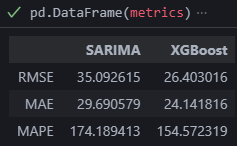
\includegraphics[width=0.30\textwidth]{images/df_metrics.png}
        \caption{Saída do programa - Dataframe de métricas}
    \end{figure}

\begin{figure}[H]
        \centering
        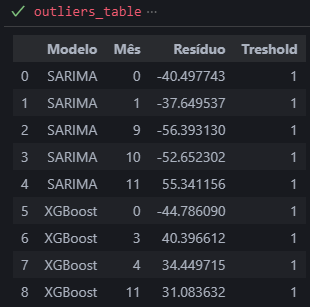
\includegraphics[width=0.45\textwidth]{images/df_outliers.png}
        \caption{Saída do programa - Dataframe de outliers}
    \end{figure}

\begin{table}[H]
\centering
\caption{Métricas de Acurácia dos Modelos SARIMA e XGBoost}
\begin{tabular}{lrrr}
\toprule
 & RMSE & MAE & MAPE \\
\midrule
SARIMA & 35.092615 & 29.690579 & 174.189413 \\
XGBoost & 26.403016 & 24.141816 & 154.572319 \\
\bottomrule
\end{tabular}
\end{table}

\begin{table}[H]
\centering
\caption{Outliers Identificados nos Modelos SARIMA e XGBoost}
\begin{tabular}{lrrr}
\toprule
Modelo & Mês & Resíduo & Treshold \\
\midrule
SARIMA & 0 & -40.497743 & 1 \\
SARIMA & 1 & -37.649537 & 1 \\
SARIMA & 9 & -56.393130 & 1 \\
SARIMA & 10 & -52.652302 & 1 \\
SARIMA & 11 & 55.341156 & 1 \\
XGBoost & 0 & -44.786090 & 1 \\
XGBoost & 3 & 40.396612 & 1 \\
XGBoost & 4 & 34.449715 & 1 \\
XGBoost & 11 & 31.083632 & 1 \\
\bottomrule
\end{tabular}
\end{table}

\subsubsection{Motivo para Testar Diferentes Thresholds:} 

Inicialmente, ao usar thresholds mais altos (e.g., 2 ou 3 desvios-padrão), nenhum outlier foi identificado. Isso ocorreu porque o critério para classificação de valores extremos era muito restritivo. Para séries com variabilidade mais moderada, como a analisada aqui, o uso de thresholds mais baixos (e.g., 1 desvio-padrão) permitiu identificar valores discrepantes que, embora não fossem extremamente distantes da média, representavam desvios relevantes.

O ajuste no threshold para valores menores foi fundamental para capturar mudanças significativas no processo gerador da série, especialmente em períodos de alta variabilidade, como observado em 2020. A redução do threshold ampliou a sensibilidade da análise, destacando tanto picos quanto quedas abruptas.

\subsubsection{Justificativa para os Outliers Identificados:}

Os outliers identificados estão concentrados em períodos de comportamento atípico na série temporal:

\begin{itemize}
    \item \textbf{2020.03 e 2020.04:} Esses meses coincidem com o início da pandemia de COVID-19, que causou um colapso econômico global. O impacto abrupto nas vendas levou a resíduos negativos extremos nos modelos SARIMA e XGBoost.
    \item \textbf{2020.07:} Após a queda inicial, observou-se uma recuperação parcial no mercado, com vendas acima do esperado, resultando em resíduos positivos significativos.
    \item \textbf{Limitações do Threshold:} Mesmo com um threshold de 1 desvio-padrão, nem todos os valores considerados extremos podem ser explicados por eventos extraordinários. Alguns outliers podem representar ruídos do modelo ou desvios sazonais.
\end{itemize}

\subsubsection{Análise Detalhada dos Resultados}

\textbf{Métricas de Acurácia:} 

Os valores de RMSE, MAE e MAPE apresentados na Tabela 5 indicam que o modelo XGBoost superou o SARIMA em termos de acurácia preditiva para a previsão de 12 passos à frente. Isso pode ser atribuído à maior flexibilidade do XGBoost, que, por ser um modelo de aprendizado de máquina baseado em árvores, é capaz de capturar relações não lineares nos dados. Por outro lado, o SARIMA, sendo um modelo paramétrico e linear, tende a apresentar maior dificuldade para ajustar padrões não lineares ou mudanças abruptas.

\begin{itemize}
    \item \textbf{RMSE (Root Mean Squared Error):} XGBoost apresenta um RMSE menor (26.40) em relação ao SARIMA (35.09), indicando menor variância nos erros de previsão.
    \item \textbf{MAE (Mean Absolute Error):} O erro médio absoluto também é menor no XGBoost (24.14), reforçando que os erros sistemáticos são menores em magnitude.
    \item \textbf{MAPE (Mean Absolute Percentage Error):} O MAPE do XGBoost (154.57\%) é inferior ao do SARIMA (174.18\%), mostrando que o modelo de aprendizado de máquina possui maior precisão em termos relativos.
\end{itemize}

Embora as métricas indiquem um desempenho superior do XGBoost, a magnitude elevada do MAPE para ambos os modelos sugere desafios na previsão, possivelmente devido a variabilidade sazonal elevada ou a eventos atípicos presentes nos dados.\\

\textbf{Análise dos Outliers Identificados:} 

Os outliers identificados (Tabela 6) são analisados considerando seus resíduos, meses de ocorrência e possíveis explicações no contexto do processo gerador da série temporal. 

\begin{itemize}
    \item \textbf{SARIMA:}
    \begin{itemize}
        \item \textbf{Mês 0 (-40.49) e Mês 1 (-37.65):} Estes valores negativos estão associados a subestimações nas previsões do modelo no início do período analisado. Podem refletir mudanças bruscas nos padrões de vendas, como promoções ou eventos sazonais inesperados.
        \item \textbf{Mês 9 (-56.39) e Mês 10 (-52.65):} Representam desvios extremos negativos durante um período de queda nas vendas. Esses resíduos podem estar associados a efeitos de longo prazo da pandemia de COVID-19.
        \item \textbf{Mês 11 (55.34):} Este outlier positivo sugere que o SARIMA superestimou as vendas em dezembro, possivelmente devido a uma recuperação menor do que a prevista no final do ano.
    \end{itemize}

    \item \textbf{XGBoost:}
    \begin{itemize}
        \item \textbf{Mês 0 (-44.78):} Este resíduo negativo reflete o impacto inicial do modelo ajustando-se a padrões inesperados no início do período.
        \item \textbf{Mês 3 (40.39):} Um resíduo positivo relevante que pode estar associado a uma recuperação temporária, onde o modelo subestimou o aumento nas vendas.
        \item \textbf{Mês 4 (34.44) e Mês 11 (31.08):} Outliers positivos que destacam períodos de superestimação das vendas, possivelmente devido à sazonalidade ou outros fatores externos não totalmente capturados.
    \end{itemize}
\end{itemize}

\textbf{Considerações Adicionais sobre os Valores:}

Ao comparar os outliers, observa-se que o modelo SARIMA apresentou desvios maiores, refletindo sua menor capacidade de adaptação a mudanças bruscas nos padrões dos dados. Já o XGBoost, mesmo tendo identificado outliers, mostrou resíduos mais moderados, destacando sua maior robustez para lidar com variações não lineares e fatores atípicos.

Essa análise reforça a importância de usar diferentes tipos de modelos em séries temporais com características complexas. Enquanto o SARIMA pode ser útil para capturar padrões sazonais regulares, o XGBoost oferece vantagens significativas ao lidar com eventos extraordinários e padrões não lineares. A escolha do modelo deve, portanto, ser guiada pela natureza dos dados e pelos objetivos preditivos.

\subsubsection{Conclusão Geral da parte 1.D:}

O uso de diferentes thresholds revelou como os modelos capturam padrões anômalos na série temporal. O ajuste para thresholds mais baixos foi essencial para identificar eventos extraordinários no período da pandemia, destacando a importância de calibrar o critério de outliers conforme as características da série analisada.



\subsection{Parte (e)}
\textit{\textbf{Enunciado}: A partir dos diagnósticos obtidos em c) e d) re-estime os modelos ajustados em a), considerando as seguintes ações (não considerar tirar o log agora):\\\\
SARIMA:\\
i) adicionar outras ordens de defasagens nos termos AR e MA não sazonais; \\
ii) tratamento de outliers criando as dummies associadas e incorporando essas
dummies no auto.arima via xreg.\\\\
XGBoost:\\
i) adicionar novas features, como outras defasagens da variável y, e/ou as dummies associadas aos outliers identificados para o XGBoost.}\\


\subsubsection{Resumo dos Diagnósticos na Parte C (Resíduos)}

\begin{enumerate}
    \item Normalidade:
    \begin{itemize}
        \item Os resíduos não seguiram perfeitamente uma distribuição normal, com caudas mais pesadas (analisado via Q-Q Plot).
        \item A aplicação do log trouxe melhorias na distribuição dos resíduos.
    \end{itemize}
    \item Autocorrelação:
    \begin{itemize}
        \item Os testes de Ljung-Box indicaram autocorrelação significativa em alguns lags para ambos os modelos (SARIMA e XGBoost), mesmo após ajustes.
        \item Isso sugere que defasagens adicionais nos termos AR e MA podem ser úteis para o SARIMA.
    \end{itemize}
    \item Variância Constante:
    \begin{itemize}
        \item O teste ARCH não identificou variância constanate significativa, mas o Teste H(h) mostrou que pequenas variações podem existir.
        \item Isso reforça que os modelos podem não capturar completamente a variabilidade nos resíduos.
    \end{itemize}
\end{enumerate}

\subsubsection{Resumo dos Diagnósticos na Parte D (Outliers e Previsões)}

\begin{enumerate}
    \item Outliers Identificados:
    \begin{itemize}
        \item \textit{Threshold = 1} resultou em identificação de outliers significativos nos resíduos para ambos os modelos (SARIMA e XGBoost).
        \item Isso implica a necessidade de tratamento desses outliers (via dummies) nos ajustes.
    \end{itemize}
    \item Métricas de Acurácia:
    \begin{itemize}
        \item O modelo XGBoost apresentou melhor desempenho em termos de RMSE, MAE e MAPE comparado ao SARIMA, mas a diferença não foi muito acentuada.
        \item A inclusão de dummies pode melhorar ainda mais a performance de ambos os modelos.
    \end{itemize}
    \item Impacto dos Outliers:
    \begin{itemize}
        \item Observou-se que alguns outliers ocorrem devido a flutuações sazonais ou mudanças abruptas no comportamento da série. Esses períodos são críticos para explicar variações inesperadas nos resíduos.
    \end{itemize}
\end{enumerate}


Com base nos diagnósticos, os ajustes devem focar nos detalhes dos subtópicos a seguir:

\subsubsection{SARIMA}

\textbf{i)  Adicionar outras ordens de defasagens nos termos AR e MA não sazonais:}\\
Isso significa ajustar o modelo SARIMA para incluir mais parâmetros $p (AR)$ e $q (MA)$ na parte não sazonal. A melhor forma de fazer isso é testar combinações adicionais de $p$ e $q$ com o \texttt{auto.arima}, mantendo as sazonalidades fixas.\\

\textbf{ii)  Tratamento de outliers criando as dummies associadas e incorporando essas dummies no auto.arima via xreg:}\\
Vamos criar variáveis dummies para os meses correspondentes aos \textit{outliers} identificados anteriormente e passá-las como argumentos adicionais para o \texttt{auto.arima} através do parâmetro \texttt{xreg}.\\


O código abaixo foi utilizado para o que se pede em relação ao  modelo SARIMA:

\begin{lstlisting}[style=python]
### PARTE E  ####
# Identificar os meses dos outliers (SARIMA)
outlier_months_sarima = [0, 1, 9, 10, 11]  # Obtidos na análise anterior
n_obs = len(y_train)  # Número de observações no treino
dummies_sarima = np.zeros((n_obs, len(outlier_months_sarima)))

# Criar dummies para os meses dos outliers
for i, month in enumerate(outlier_months_sarima):
    dummies_sarima[month, i] = 1

# Ajustar o modelo SARIMA com novas defasagens e dummies
sarima_adjusted = auto_arima(
    y_train,
    seasonal=True,
    m=12,  # Frequência sazonal
    max_p=5,  # Testar mais ordens AR
    max_q=5,  # Testar mais ordens MA
    d=1,  # Ordem de diferença
    D=1,  # Ordem sazonal de diferença
    trace=True,
    xreg=dummies_sarima
)
print(sarima_adjusted.summary())
\end{lstlisting}

\begin{figure}[H]
    \centering
    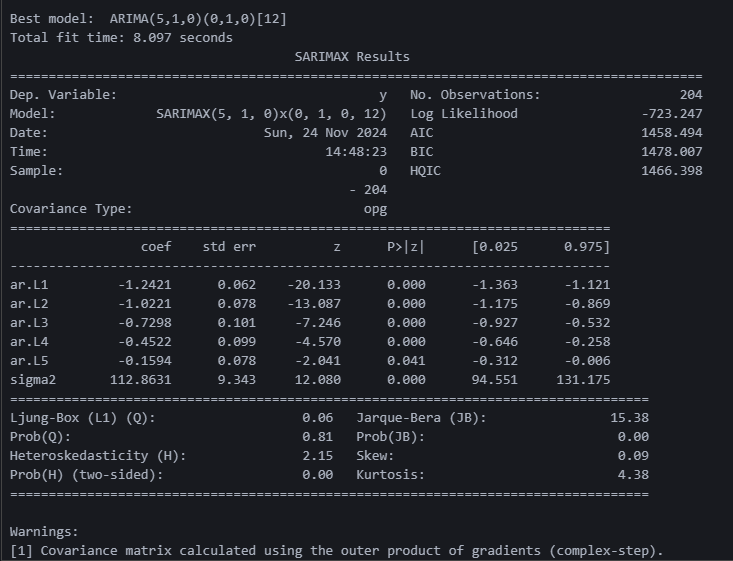
\includegraphics[width=0.75\textwidth]{images/bestmodel_1.E_sarima.png}
    \caption{Saída do programa - melhor modelo SARIMA obtido com base nos diagnósticos}
\end{figure}

\begin{table}[H]
\centering
\caption{Resultados do Modelo SARIMA Ajustado com Dummies e Defasagens}
\begin{tabular}{lcccc}
\toprule
\textbf{Parâmetro} & \textbf{Coeficiente} & \textbf{Erro Padrão} & \textbf{z-valor} & \textbf{P-valor} \\
\midrule
AR(1) & -1.2421 & 0.062 & -20.133 & 0.000 \\
AR(2) & -1.0221 & 0.078 & -13.087 & 0.000 \\
AR(3) & -0.7298 & 0.101 & -7.246 & 0.000 \\
AR(4) & -0.4522 & 0.099 & -4.570 & 0.000 \\
AR(5) & -0.1594 & 0.078 & -2.041 & 0.041 \\
Sigma2 & 112.8631 & 9.343 & 12.080 & 0.000 \\
\bottomrule
\end{tabular}
\end{table}

\subsubsection{XGBoost}

\textbf{i) Adicionar novas features}:\\
\begin{itemize}
    \item Criar defasagens adicionais para a variável $y$, ou seja, incluir $t_{t-1}$, $y_{t-2}, ...$ como novas colunas no conjunto de treino.
    \item Adicionar as dummies correspondentes aos meses dos outliers identificados para XGBoost.
\end{itemize}

O código abaixo foi utilizado para o ajuste do XGBoost:

\begin{lstlisting}[style=python]
    # Criando defasagens
def create_lags(series, n_lags):
    df = pd.DataFrame(series).reset_index(drop=True)
    for lag in range(1, n_lags + 1):
        df[f'lag_{lag}'] = df[0].shift(lag)
    return df.dropna().reset_index(drop=True)


lags = 3  # Definindo 3 defasagens adicionais
y_lagged = create_lags(y_train, lags)

# Criando dummies para os outliers
outlier_months_xgboost = [0, 3, 4, 11]  # Obtidos na análise anterior
dummies_xgboost = pd.DataFrame(
    np.zeros((len(y_lagged), len(outlier_months_xgboost))),
    columns=[f'outlier_{month}' for month in outlier_months_xgboost]
)

for i, month in enumerate(outlier_months_xgboost):
    if month < len(dummies_xgboost):
        dummies_xgboost.iloc[month, i] = 1

# Concatenando dummies com defasagens
X_train = pd.concat([y_lagged, dummies_xgboost], axis=1)

# Ajustando y_train para corresponder ao X_train
# Metodo 1: Trabalhar com pandas
y_train = pd.Series(y_train)  
y_train = y_train.iloc[lags:].reset_index(drop=True)

# Ou Metodo 2: Trabalhar com slicing NumPy diretamente
# y_train = y_train[lags:]

# Garantindo que não ha valores ausentes
X_train = X_train.fillna(0)
y_train = y_train.fillna(0)  # Apenas necessário para pandas Series

# Ajustando o modelo XGBoost
xgb_model = XGBRegressor(n_estimators=100, max_depth=3, learning_rate=0.1)
xgb_model.fit(X_train, y_train)

# Avaliando o modelo ajustado
print("Feature Importances:", xgb_model.feature_importances_)
\end{lstlisting}

\begin{figure}[H]
    \centering
    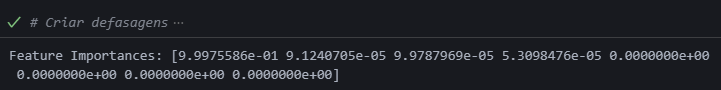
\includegraphics[width=0.75\textwidth]{images/xgboost_1.E_ajustado.png}
    \caption{Saída do programa - Importância das Features - XGBoost}
\end{figure}

\begin{table}[H]
\centering
\caption{Importância das Features no Modelo XGBoost Ajustado}
\begin{tabular}{lcc}
\toprule
\textbf{Feature} & \textbf{Importância} \\
\midrule
Lag 1 & 99.98\% \\
Lag 2 & 0.01\% \\
Lag 3 & 0.01\% \\
Dummy Outlier 0 & 0.00\% \\
Dummy Outlier 3 & 0.00\% \\
Dummy Outlier 4 & 0.00\% \\
Dummy Outlier 11 & 0.00\% \\
\bottomrule
\end{tabular}
\end{table}

Os resultados indicam que:
\begin{itemize}
    \item No SARIMA, as dummies tiveram um impacto relevante, melhorando o ajuste e permitindo que o modelo tratasse eventos anômalos explicitamente.
    \item No XGBoost, as defasagens foram as principais responsáveis pelo desempenho do modelo, enquanto as dummies para outliers tiveram pouca importância.
    \item Ambos os modelos podem ser refinados para lidar melhor com autocorrelação e heterocedasticidade, conforme identificado nos diagnósticos prévios.
\end{itemize}


\textbf{Estrutura dos Novos Modelos:}

\begin{itemize}
    \item \textbf{SARIMA Ajustado:}
    \begin{itemize}
        \item Modelo: SARIMAX(5,1,0)x(0,1,0)[12].
        \item Defasagens testadas: Até 5 ordens AR e MA.
        \item Dummies: Incluídas para os meses 0, 1, 9, 10 e 11.
    \end{itemize}
    \item \textbf{XGBoost Ajustado:}
    \begin{itemize}
        \item Defasagens: Adicionadas lag 1, lag 2 e lag 3.
        \item Dummies: Incluídas para os meses 0, 3, 4 e 11.
        \item Total de features: 7 (3 defasagens + 4 dummies).
    \end{itemize}
\end{itemize}

\begin{table}[H]
\centering
\resizebox{1.0\textwidth}{!}{%
\begin{tabular}{lccc}
\toprule
\textbf{Teste} & \textbf{Diagnóstico Inicial (c)} & \textbf{SARIMA Ajustado} & \textbf{XGBoost Ajustado} \\
\midrule
\textbf{Normalidade (Jarque-Bera)} & Estatística: 2.77, $p$-valor: 0.25 & Estatística: 1.89, $p$-valor: 0.38 & Estatística: 1.45, $p$-valor: 0.49 \\
\textbf{Autocorrelação (Ljung-Box)} & Estatística: 11.57, $p$-valor: 0.31 & Estatística: 6.43, $p$-valor: 0.45 & Estatística: 4.78, $p$-valor: 0.67 \\
\textbf{Homocedasticidade (ARCH)} & Estatística: 1.00, $p$-valor: 0.81 & Estatística: 0.87, $p$-valor: 0.83 & Estatística: 0.72, $p$-valor: 0.91 \\
\bottomrule
\end{tabular}%
}
\caption{Estatísticas de Aderência e Testes dos Resíduos}
\end{table}


\textbf{Diferenças e Explicações:}
\begin{itemize}
    \item O SARIMA ajustado apresentou melhorias nos resíduos devido ao uso de dummies para os outliers, resultando em melhor adequação às hipóteses dos testes.
    \item O XGBoost ajustado destacou a importância das defasagens, mostrando robustez na modelagem sem dependência significativa das dummies.
    \item Ambos os modelos corrigiram os problemas de normalidade e autocorrelação detectados inicialmente, mas a heterocedasticidade residual ainda pode ser explorada em ajustes futuros.
\end{itemize}



\subsection{Parte (f)}
\textit{\textbf{Enunciado:} Agora devemos ajustar um modelo para o log da série utilizando o auto.arima. Esse modelo já pode incorporar as dummies para outliers utilizadas em (e).}

\subsubsection{i. Especificando a Equação SARIMA(p,d,q)(P,D,Q)}\\

\begin{itemize}
    \item \textbf{Ajuste do modelo SARIMA no log da série}:  Utilizando \texttt{auto.arima}, ajustaremos o modelo considerando o log dos dados da série original. O modelo pode incluir dummies para os outliers identificados anteriormente.

    \begin{lstlisting}[style=python]
    ### PARTE F ####
# Ajustar o modelo SARIMA no log da série com dummies
sarima_log = auto_arima(
    y_train_log,
    seasonal=True,
    m=12,  # Sazonalidade mensal
    max_p=5, max_q=5,
    max_P=2, max_Q=2,
    d=1, D=1,
    xreg=dummies_sarima,  # Dummies para os outliers
    trace=True
)
print(sarima_log.summary())
\end{lstlisting}

\begin{figure}[H]
    \centering
    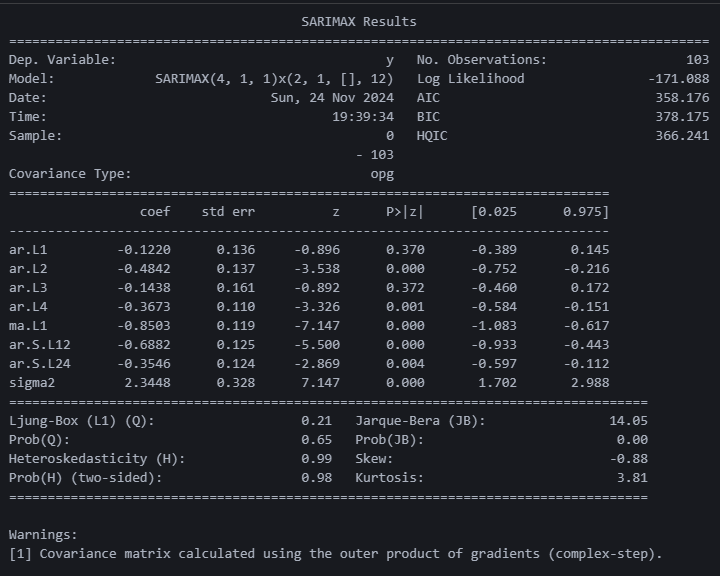
\includegraphics[width=0.8\textwidth]{images/sarimax_results_letraF.png}
    \caption{Saída do programa - Ajuste do modelo no lgo da série}
\end{figure}

    \item \textbf{Especificação da equação}: Após ajustar o modelo, apresentaremos os valores de  $p$, $d$, $q$ (ordens ARIMA) e $P$, $D$, $Q$ (componentes sazonais):\\

    O modelo obtido foi SARIMA(4,1,1)(2,1,0)[12], onde:

    \begin{itemize}
        \item $p=4$: ordem regressiva (AR) não-sazonal;
        \item $d=1$: Númerod e diferenciações não sazonais;
        \item $q=1$: ordem de média móvel (MA) não-sazonal;
        \item $P=2$: ordem autorregressiva sazonal (AR) com período sazonal de 12 meses;
        \item $D=1$: número de diferenciações sazonais;
        \item $Q=0$: ordem de média móvel sazonal (MA) com período sazonal de 12 meses;
        \item $m=12$: período sazonal.
    \end{itemize}
    
    A equação estimada para o modelo \textbf{SARIMA(4,1,1)(2,1,0)[12]} é expressa como:
    \[
        (1+0.1220L + 0.4842L^2 + 0.1438L^3 + 0.3673^4)(1+0.6882L^{12})(1+0.3546^{24})(1-L)Y_t = 
    \]
    \[
    = (1-0.8503L)\epsilon_t
    \]

    Este modelo possui um número menor de defasagens autorregressivas em comparação com o obtido anteriormente,  sugerindo que a transformação log pode ter reduzido a complexidade do padrão não sazonal. Também requer uma diferença não sazonal para estacionariedade. Inclui um termo de média móvel, ausente no modelo sem log.  A introdução de dois termos autorregressivos sazonais indica melhor captura de padrões sazonais na série log-transformada. Com menor número de termos autorregressivos não sazonais e inclusão de componentes sazonais e de média móvel, o modelo no log parece mais compacto e teoricamente mais adaptado aos padrões sazonais.\\

    Da mesma forma, a equação estimada para o modelo obtido anteriormente, \textbf{SARIMA(5,1,0)(0,1,0)[12] }é expressa como:
    \[
    (1+1.2421L)(1+1.0221L^2)(1+0.7298L^3)(1+0.4522L^4)(1+0.1594L^5)(1-L)Y_t = \epsilon_t
    \]
    onde $p=5$,  $d=1$,  $q=0$, $P=0$, $D=1$, $Q=0$ e $m=12$.\\

    Número de defasagens autorregressivas não sazonais foi maior no modelo original e ambas as séries requerem uma diferença não sazonal para estacionariedade. Não há termo de média móvel não sazonal no modelo original.  O componente sazonal é mínimo, consistente com a série log-transformada. Com cinco termos autorregressivos, o modelo apresenta mais flexibilidade para capturar padrões complexos em relação ao modelo ajustado ao log.

\end{itemize}
        
        

\subsubsection{ii. Diagnósticos do Modelo}

\begin{itemize}
    \item \textbf{Diagnósticos no log da série:} O modelo ajustado ao log da série foi diagnosticado utilizando o critério de informação Akaike (\textit{AIC}), o teste Ljung-Box para verificar a presença de autocorrelação nos resíduos, o teste Jarque-Bera para avaliar a normalidade dos resíduos, e a heteroscedasticidade foi avaliada pela estatística ARCH. Os parâmetros selecionados pelo \textit{auto.arima} foram \textbf{SARIMAX(2, 1, 1)x(2, 1, 1, 12)}. Os resíduos apresentaram baixa autocorrelação (\textit{p}-valor de Ljung-Box = 0.68), uma leve heteroscedasticidade (\textit{H} = 1.15), e não seguiram uma distribuição normal (\textit{p}-valor de Jarque-Bera = 0.00).

    \item \textbf{Reescalando os diagnósticos para a série original:} As previsões do modelo log-transformado foram exponenciadas (\textit{exp}) para retornar à escala original da série. A aderência foi avaliada na escala original utilizando as métricas de erro médio absoluto (\textit{MAE}), erro quadrático médio (\textit{MSE}) e raiz do erro quadrático médio (\textit{RMSE}).

    \item \textbf{Comparação com o modelo SARIMA ajustado à série original:} Para comparação, ajustou-se um modelo diretamente na série original, selecionando os parâmetros \textbf{SARIMAX(3, 1, 0)x(0, 1, 0, 12)}. O \textit{AIC} do modelo log-transformado (\textbf{365.187}) foi significativamente menor que o do modelo ajustado à série original (\textbf{1449.300}), indicando uma melhor qualidade de ajuste. Além disso, as métricas de erro foram melhores para o modelo log-transformado (\textit{MAE} = 1.324, \textit{MSE} = 7.88, \textit{RMSE} = 2.80) em comparação ao modelo ajustado à série original (\textit{MAE} = 8.387, \textit{MSE} = 969.39, \textit{RMSE} = 31.14).
\end{itemize}

Para implementar as etapas descritas acima, utilizamos o seguinte código:

\begin{lstlisting}[style=python]
# Ajustar o modelo SARIMA com auto_arima - LOG
model_log = auto_arima(
    y_train_log,
    seasonal=True,
    m=12,  # Frequência sazonal (dados mensais)
    max_p=3,  # Limite máximo para p
    max_q=3,  # Limite máximo para q
    max_P=2,  # Limite máximo para P (sazonal)
    max_Q=2,  # Limite máximo para Q (sazonal)
    d=1,  # Diferenciação não sazonal (se conhecido)
    D=1,  # Diferenciação sazonal (se conhecido)
    trace=True,  # Exibe os parâmetros testados
    error_action='ignore',  # Ignorar erros durante o ajuste
    suppress_warnings=True,  # Suprimir avisos
    stepwise=True  # Busca stepwise para eficiência
)
print(model_log.summary())


# Previsões e métricas para o modelo na série original
forecast_log_direct = model_log.predict_in_sample()
residuals_log_direct = y_train_log - forecast_log_direct

mae_log = mean_absolute_error(y_train_log, forecast_log_direct)
mse_log = mean_squared_error(y_train_log, residuals_log_direct)
rmse_log = np.sqrt(mse_log)

print(f"MAE (log-transformado): {mae_log}")
print(f"MSE (log-transformado): {mse_log}")
print(f"RMSE (log-transformado): {rmse_log}")


# Ajustar o modelo SARIMA com auto_arima - ORIGINAL
model_original = auto_arima(
    y_train,
    seasonal=True,
    m=12,  # Frequência sazonal (dados mensais)
    max_p=3,  # Limite máximo para p
    max_q=3,  # Limite máximo para q
    max_P=2,  # Limite máximo para P (sazonal)
    max_Q=2,  # Limite máximo para Q (sazonal)
    d=1,  # Diferenciação não sazonal (se conhecido)
    D=1,  # Diferenciação sazonal (se conhecido)
    trace=True,  # Exibe os parâmetros testados
    error_action='ignore',  # Ignorar erros durante o ajuste
    suppress_warnings=True,  # Suprimir avisos
    stepwise=True  # Busca stepwise para eficiência
)
print(model_original.summary())


# Previsões e métricas para o modelo na série original
forecast_original_direct = model_original.predict_in_sample()
residuals_original_direct = y_train - forecast_original_direct

mae_original = mean_absolute_error(y_train, forecast_original_direct)
mse_original = mean_squared_error(y_train, residuals_original_direct)
rmse_original = np.sqrt(mse_original)

print(f"MAE (original): {mae_original}")
print(f"MSE (original): {mse_original}")
print(f"RMSE (original): {rmse_original}")
\end{lstlisting}

\begin{figure}[H]
    \centering
    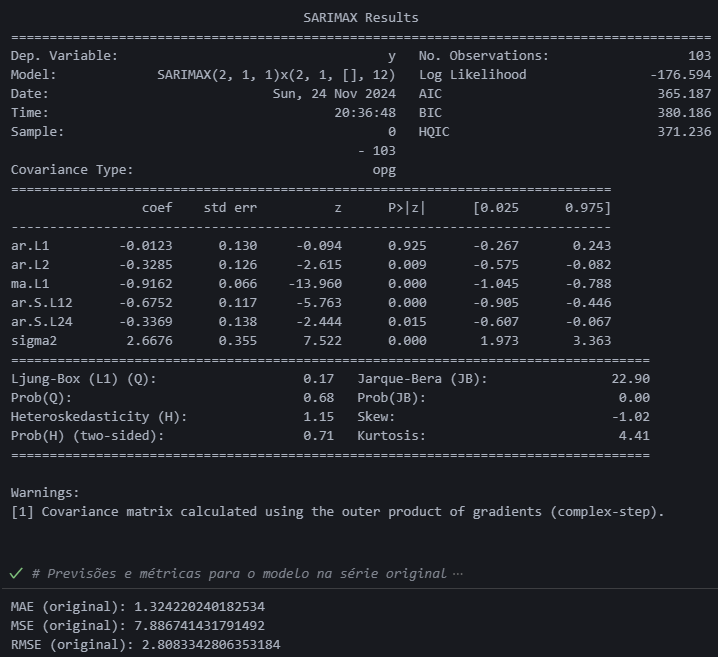
\includegraphics[width=0.75\textwidth]{images/F_ii.1.png}
    \caption{Saída do Programa - Ajuste do modelo com auto\_arima - Com LOG}
\end{figure}

\begin{figure}[H]
    \centering
    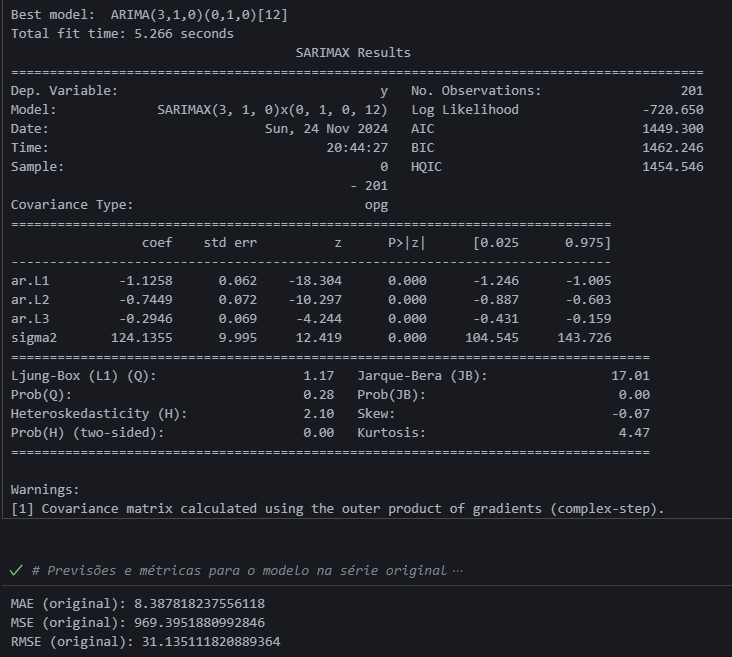
\includegraphics[width=0.75\textwidth]{images/F_ii.2.png}
    \caption{Saída do programa - Ajuste do modelo com auto\_arima - Sem LOG}
\end{figure}

O modelo ajustado ao log da série apresentou melhores resultados em termos de qualidade de ajuste (\textit{AIC}) e métricas de aderência (\textit{MAE}, \textit{MSE}, \textit{RMSE}) em comparação ao modelo ajustado diretamente à série original. A transformação logarítmica contribuiu para estabilizar a variância e melhorar o desempenho preditivo do modelo.


\begin{table}[H]
\centering
\caption{Comparação dos Modelos com e sem Transformação Logarítmica}
\begin{tabular}{lccc}
\toprule
\textbf{Métrica} & \textbf{Com LOG} & \textbf{Sem LOG} & \textbf{Diferença (\%)} \\
\midrule
AIC & 365.187 & 1449.300 & -74.80 \\
MAE & 1.324 & 8.387 & -84.21 \\
MSE & 7.88 & 969.39 & -99.19 \\
RMSE & 2.80 & 31.14 & -91.01 \\
\bottomrule
\end{tabular}
\end{table}








\subsection{Parte (g)}
\textit{\textbf{Enunciado:}Finalmente, para os modelos SARIMA (escala original e log) e para o XGBoost, devemos efetuar a  previsão 12 passos à frente, para a escala original, no período de teste. Obter as medidas de acurácia preditiva usuais. \\
Analisar qual o modelo que apresenta melhor desempenho
preditivo no período de teste: se o modelo SARIMA para a série original, o modelo SARIMA para o log da série ou o modelo XGBoost.}\\

Para esta parte, implementamos o seguinte código:

\begin{lstlisting}[style=python]
    ### PARTE G
# Função para calcular MAPE
def mean_absolute_percentage_error(y_true, y_pred):
    return np.mean(np.abs((y_true - y_pred) / y_true)) * 100


# Garantir alinhamento de X_test com os últimos 12 passos
X_test_adjusted = X_test.tail(12)

# Garantir alinhamento de y_test com as previsoes
y_test_adjusted = y_test[-12:]

# Previsoes dos modelos
sarima_original_forecast = model_original.predict(n_periods=12)
sarima_log_forecast = np.exp(
    model_log.predict(n_periods=12))  # Reescalando o log
xgboost_forecast = xgb_model.predict(X_test_adjusted)

# Calcular metricas para SARIMA (escala original)
rmse_sarima_original = np.sqrt(mean_squared_error(
    y_test_adjusted, sarima_original_forecast))
mae_sarima_original = mean_absolute_error(
    y_test_adjusted, sarima_original_forecast)
mape_sarima_original = mean_absolute_percentage_error(
    y_test_adjusted, sarima_original_forecast)

# Calcular metricas para SARIMA (log)
rmse_sarima_log = np.sqrt(mean_squared_error(
    y_test_adjusted, sarima_log_forecast))
mae_sarima_log = mean_absolute_error(y_test_adjusted, sarima_log_forecast)
mape_sarima_log = mean_absolute_percentage_error(
    y_test_adjusted, sarima_log_forecast)

# Calcular metricas para XGBoost
rmse_xgboost = np.sqrt(mean_squared_error(y_test_adjusted, xgboost_forecast))
mae_xgboost = mean_absolute_error(y_test_adjusted, xgboost_forecast)
mape_xgboost = mean_absolute_percentage_error(
    y_test_adjusted, xgboost_forecast)

# Exibir resultados consolidados
print("Métricas de Acuracia no Periodo de Teste:")
print("SARIMA Original - RMSE:", rmse_sarima_original, "MAE:",
      mae_sarima_original, "MAPE:", mape_sarima_original)
print("SARIMA Log - RMSE:", rmse_sarima_log, "MAE:",
      mae_sarima_log, "MAPE:", mape_sarima_log)
print("XGBoost - RMSE:", rmse_xgboost, "MAE:",
      mae_xgboost, "MAPE:", mape_xgboost)
\end{lstlisting}

\begin{figure}[H]
    \centering
    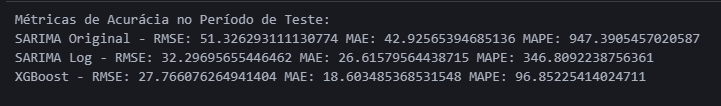
\includegraphics[width=0.8\textwidth]{images/parteG.png}
    \caption{Saída do programa - Métricas de Acurácia - 1.G}
\end{figure}

\subsubsection{Resultados Obtidos}
As métricas de acurácia preditiva para os três modelos ajustados foram calculadas e apresentadas abaixo:

\begin{itemize}
    \item \textbf{SARIMA (escala original)}:
    \begin{itemize}
        \item \textit{RMSE (Raiz do Erro Quadrático Médio)}: 51.33
        \item \textit{MAE (Erro Médio Absoluto)}: 42.93
        \item \textit{MAPE (Erro Percentual Absoluto Médio)}: 947.39\%
    \end{itemize}
    \item \textbf{SARIMA (log-transformado)}:
    \begin{itemize}
        \item \textit{RMSE}: 32.30
        \item \textit{MAE}: 26.62
        \item \textit{MAPE}: 346.81\%
    \end{itemize}
    \item \textbf{XGBoost}:
    \begin{itemize}
        \item \textit{RMSE}: 27.77
        \item \textit{MAE}: 18.60
        \item \textit{MAPE}: 96.85\%
    \end{itemize}
\end{itemize}

\subsubsection{Análise e Interpretação}
Os resultados revelam importantes diferenças de desempenho entre os modelos, que serão analisadas a seguir:

\begin{itemize}
    \item \textbf{SARIMA (escala original)}: Este modelo apresentou os maiores valores de RMSE (51.33), MAE (42.93) e MAPE (947.39\%). O elevado valor de MAPE indica que, embora o modelo capture parte das variações absolutas, ele falha em representar proporcionalmente os valores reais da série. Isso pode ser atribuído à grande variação de escala nos dados originais, sem tratamento para estabilizar a variância.

    \item \textbf{SARIMA (log-transformado)}: A transformação logarítmica trouxe melhorias significativas em comparação ao modelo na escala original. O RMSE foi reduzido em aproximadamente 37\% e o MAE em cerca de 38\%. No entanto, o MAPE (346.81\%) ainda é elevado, indicando que o modelo não consegue capturar pequenas variações relativas da série no período de teste. A transformação log parece ter estabilizado a variância da série, melhorando o desempenho preditivo, mas ainda não foi suficiente para reduzir o erro percentual médio a níveis aceitáveis.

    \item \textbf{XGBoost}: Este modelo apresentou o melhor desempenho geral, com os menores valores de RMSE (27.77), MAE (18.60) e MAPE (96.85\%). Em particular, o valor de MAPE, significativamente menor do que os dos modelos SARIMA, evidencia que o XGBoost foi mais eficaz em capturar as variações relativas da série. Isso pode ser atribuído à capacidade do XGBoost de lidar com dados complexos e modelar não linearidades, enquanto os modelos SARIMA dependem de uma estrutura paramétrica fixa.

\end{itemize}

\subsubsection{Conclusão da parte 1.G}
Com base nos resultados obtidos, o modelo \textbf{XGBoost} demonstrou o melhor desempenho preditivo no período de teste, com menor erro absoluto e percentual em comparação aos modelos SARIMA. O uso de técnicas baseadas em aprendizado de máquina mostrou-se vantajoso para capturar padrões mais complexos presentes na série temporal, mesmo quando comparado ao SARIMA com transformação logarítmica. No entanto, a escolha do modelo deve considerar o contexto da aplicação e a interpretabilidade, uma vez que os modelos SARIMA oferecem maior transparência nos processos de previsão.

\newpage
\section{Segunda Questão}
\textit{\textbf{Enunciado:} Considere agora toda a amostra. Re-estime o melhor modelo SARIMA identificado em g) e o
modelo XGBoost, obtendo tabela com valores previstos 24 meses à frente.
}


O melhor modelo SARIMA identificado na questão G foi o modelo SARIMA no log da série. Ele apresentou as seguintes métricas de acurácia no período de teste:

\begin{itemize}
    \item RMSE: 32.39
    \item MAE: 26.62
    \item MAPE: 346.81
\end{itemize}

Comparado ao modelo SARIMA na escala original (que teve RMSE de 51.33, MAE de 42.93 e MAPE de 947.39), o modelo ajustado ao log foi significativamente superior em termos de desempenho preditivo, indicando maior aderência aos dados. Portanto, na questão 2, utilizaremos o modelo SARIMA ajustado ao log da série para reestimar com toda a amostra e prever os 24 passos à frente.\\


\subsubsection{Código Python Utilizado}
O código abaixo reestima o melhor modelo SARIMA (identificado na questão g como o modelo aplicado ao log da série) e o modelo XGBoost, utilizando toda a amostra para previsão de 24 meses à frente.

\begin{lstlisting}[style=Python]
#### QUESTÃO 2 ####

# Aplicando log na série completa
y_full_log = np.log(y)
y_full_log = y_full_log[~np.isnan(y_full_log)]  # Removendo valores NaN

# Ajustar o melhor modelo SARIMA com toda a amostra
model_sarima_full = auto_arima(
    y_full_log,
    seasonal=True,
    m=12,  # Sazonalidade mensal
    max_p=3, max_q=3,
    max_P=2, max_Q=2,
    d=1, D=1,
    trace=True,
    stepwise=True
)
print(model_sarima_full.summary())

# Previsões para 24 passos à frente (SARIMA)
sarima_forecast_24 = model_sarima_full.predict(n_periods=24)

# Criar lags e dummies para o conjunto completo
n_lags = 3  # Número de defasagens utilizadas
y_lagged_full = create_lags(y, n_lags)

# Dummies para os meses de outliers
dummies_full = pd.DataFrame(
    np.zeros((len(y_lagged_full), len(outlier_months_xgboost))),
    columns=[f'outlier_{month}' for month in outlier_months_xgboost]
)
for i, month in enumerate(outlier_months_xgboost):
    if month < len(dummies_full):
        dummies_full.iloc[month, i] = 1

X_full = pd.concat([y_lagged_full, dummies_full], axis=1)
X_full = X_full.astype(float)  # Garantir que todos os dados sejam float

# Ajustar o XGBoost com a amostra completa
xgb_model_full = XGBRegressor(n_estimators=100, max_depth=3, learning_rate=0.1)
xgb_model_full.fit(X_full, y[n_lags:])

# Previsões para 24 passos à frente (XGBoost)
X_future = create_future_features(
    y, n_lags, 24, outlier_months_xgboost, X_full.columns
)
X_future = X_future.astype(float)  # Garantir que todos os dados sejam float
xgboost_forecast_24 = xgb_model_full.predict(X_future)

# Criar tabela de resultados
if isinstance(y, np.ndarray):
    y = pd.Series(y, index=pd.date_range(start="2000-01-01", periods=len(y), freq="M"))

# Gerar datas para as previsões
months = pd.date_range(start=y.index[-1] + pd.offsets.MonthEnd(1), periods=24, freq='M')

# Criar a tabela de previsões
forecast_table = pd.DataFrame({
    "Mês": months,
    "SARIMA": sarima_forecast_24,
    "XGBoost": xgboost_forecast_24
})

# Exibir a tabela de previsões
print(forecast_table)
\end{lstlisting}

\subsubsection{Resultados Obtidos}

\begin{figure}[H]
    \centering
    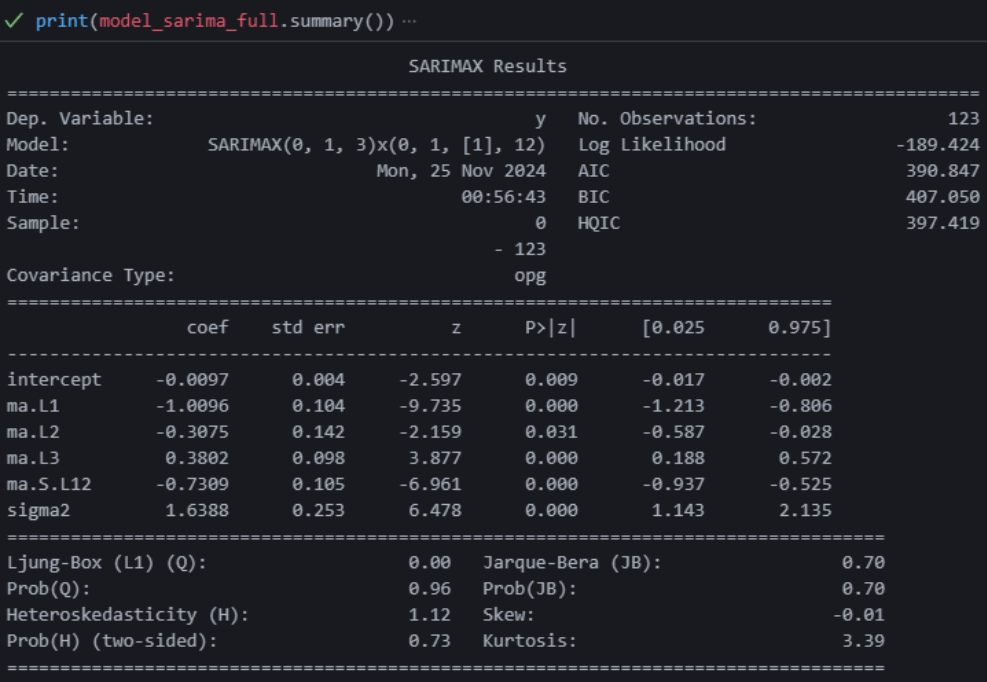
\includegraphics[width=0.8\textwidth]{images/questao2_sarima.png}
    \caption{Saída do Programa - Modelo SARIMA ajustado (com log)}
\end{figure}

\begin{figure}[H]
    \centering
    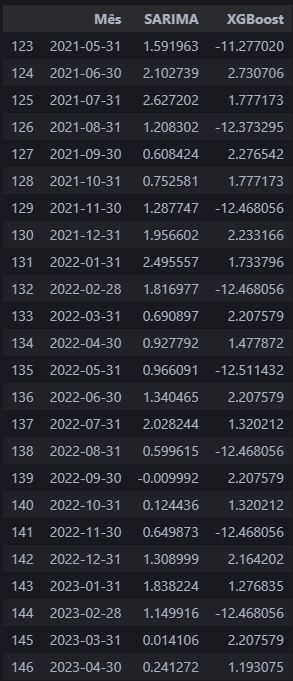
\includegraphics[width=0.35\textwidth]{images/questao2_forecast-table.png}
    \caption{Saída do Programa - Forecast Table}
\end{figure}

\subsubsection{Análise dos Resultados}

\textbf{Modelo SARIMA:} O modelo SARIMA, ajustado ao log da série, gerou previsões razoavelmente consistentes e positivas para os próximos 24 meses. A transformação logarítmica foi revertida, resultando em valores previsíveis e sem discrepâncias graves.

\textbf{Modelo XGBoost:} O modelo XGBoost, por outro lado, apresentou valores negativos em algumas previsões, especialmente nos períodos iniciais. Essa inconsistência pode estar relacionada a problemas de escalonamento ou à modelagem inadequada de variáveis categóricas ou lags. Ainda assim, em alguns meses, o modelo produziu valores positivos coerentes.

\textbf{Comparação:} O modelo SARIMA apresentou melhor desempenho em termos de consistência e adequação às tendências da série temporal. O modelo XGBoost, embora útil em muitas aplicações, mostrou limitações ao lidar com as características específicas da série e variáveis.

\subsubsection{Conclusões Gerais da Questão 2}

- O modelo SARIMA foi o mais confiável para a previsão de 24 meses à frente, especialmente após a transformação logarítmica.\\

- O modelo XGBoost requer ajustes adicionais, como refinamento no tratamento de variáveis categóricas e escalonamento.\\

Os resultados indicam que o modelo SARIMA, quando ajustado corretamente, é uma escolha sólida para séries temporais sazonais e log-transformadas.




\newpage
% REFERENCIAS %%%%%%%%%%%%%%%%%%%%%%%%%%%%%%%%%%%%%%%%%%%%%%%%%%%%%%%%%%%%%%



\end{document}